\documentclass{report}
\usepackage{amsmath}
\usepackage{amsfonts} 
\usepackage{physics} 
\usepackage{rotating}
\usepackage{enumitem}
\setlength{\headheight}{15pt}
\usepackage[italian]{varioref}
\usepackage{hyperref}
\usepackage{steinmetz}
\hypersetup{colorlinks=true, linkcolor=magenta, citecolor=green, urlcolor=blue} 
\usepackage{mathtools}
\hypersetup{linktoc=page}
\usepackage{extramarks}
\usepackage{amssymb}
\usepackage{fancyhdr}
\usepackage{float}
\usepackage{geometry}
 \geometry{
 a4paper,
 total={190mm,257mm},
 left=15mm,
 right=15mm,
 top=20mm,
 }
\usepackage{graphicx}
\usepackage{cancel}
\graphicspath{ {./images/} }
\newcommand{\R}{\mathbb{R}}
\newcommand{\N}{\mathbb{N}}
\usepackage{amsthm}
\usepackage{etoolbox}
\newtheoremstyle{break}
  {\topsep}{\topsep}%
  {\itshape}{}%
  {\bfseries}{}%
  {\newline}{}%
\theoremstyle{break}
\newtheorem{definition}{Definition}[section]
\newtheorem{example}{Example}[section]
\newtheorem{hw}{Exercise}[section]
\newtheorem{theorem}{Theorem}[section]
\BeforeBeginEnvironment{minipage}{\medskip}
\AfterEndEnvironment{minipage}{\medskip}
\usepackage{tocloft}

\usepackage{indentfirst}
\usepackage{tikz}
\usepackage{afterpage}
\numberwithin{equation}{section}
\newcommand\blankpage{%
    \null
    \thispagestyle{empty}%
    \addtocounter{page}{-1}%
    \newpage}
\newcommand\blankpagewnumber{%
    \null
    \newpage}
\newcommand{\T}{\mathcal{T}}
\newcommand{\U}{\mathcal{U}}
\renewcommand{\L}{\mathcal{L}}
\usepackage{blkarray, bigstrut}
\usepackage[T1]{fontenc}
% --- Macro \xvec
\makeatletter
\newlength\xvec@height%
\newlength\xvec@depth%
\newlength\xvec@width%
\newcommand{\xvec}[2][]{%
  \ifmmode%
    \settoheight{\xvec@height}{$#2$}%
    \settodepth{\xvec@depth}{$#2$}%
    \settowidth{\xvec@width}{$#2$}%
  \else%
    \settoheight{\xvec@height}{#2}%
    \settodepth{\xvec@depth}{#2}%
    \settowidth{\xvec@width}{#2}%
  \fi%
  \def\xvec@arg{#1}%
  \def\xvec@dd{:}%
  \def\xvec@d{.}%
  \raisebox{.2ex}{\raisebox{\xvec@height}{\rlap{%
    \kern.05em%  (Because left edge of drawing is at .05em)
    \begin{tikzpicture}[scale=1]
    \pgfsetroundcap
    \draw (.05em,0)--(\xvec@width-.05em,0);
    \draw (\xvec@width-.05em,0)--(\xvec@width-.15em, .075em);
    \draw (\xvec@width-.05em,0)--(\xvec@width-.15em,-.075em);
    \ifx\xvec@arg\xvec@d%
      \fill(\xvec@width*.45,.5ex) circle (.5pt);%
    \else\ifx\xvec@arg\xvec@dd%
      \fill(\xvec@width*.30,.5ex) circle (.5pt);%
      \fill(\xvec@width*.65,.5ex) circle (.5pt);%
    \fi\fi%
    \end{tikzpicture}%
  }}}%
  #2%
}
\makeatother

% --- Override \vec with an invocation of \xvec.
\let\stdvec\vec
\renewcommand{\vec}[1]{\xvec[]{#1}}
% --- Define \dvec and \ddvec for dotted and double-dotted vectors.
\newcommand{\dvec}[1]{\xvec[.]{#1}}
\newcommand{\ddvec}[1]{\xvec[:]{#1}}

\bibliographystyle{plain} 

\usepackage{algpseudocode}
\begin{document}
\afterpage{\blankpage}
\begin{titlepage}
\begin{center}
\huge Master's degree in Computer Engineering for Robotics and Smart Industry
\end{center}
\vspace*{\fill}
\begin{center}
\textbf{\Huge Robotics, Vision and Control}
\end{center}
\begin{center}
Report on the assignments given during the 2021/2022 a.y.
\end{center}
\vspace*{\fill}
\begin{center}
\begin{minipage}{0.4\textwidth}
\begin{flushleft}
Author: Lorenzo Busellato, VR472249\\
email: lorenzo.busellato\_02@studenti.univr.it
\end{flushleft}
\end{minipage}
\begin{minipage}{0.5\textwidth}
\begin{flushright}

\includegraphics[keepaspectratio,width=0.6\textwidth]{logo}
\end{flushright}
\end{minipage}

\end{center}
\vspace{1cm}
\end{titlepage}


\afterpage{\blankpage}
\thispagestyle{empty}
\setcounter{page}{0}
\pagenumbering{gobble}
\renewcommand{\cftsecleader}{\cftdotfill{\cftdotsep}}
\setcounter{tocdepth}{2}
\tableofcontents
\clearpage

\fancyhead[R]{}
\fancyhead[L]{}
\pagestyle{fancy}
\pagenumbering{arabic}

\chapter{Robotics}

\section{Assignment 1}

\subsection{3D model creation using Zephyr}

The object chosen for the assignment was a plastic statue of an angel.

\begin{figure}[h]
\centering
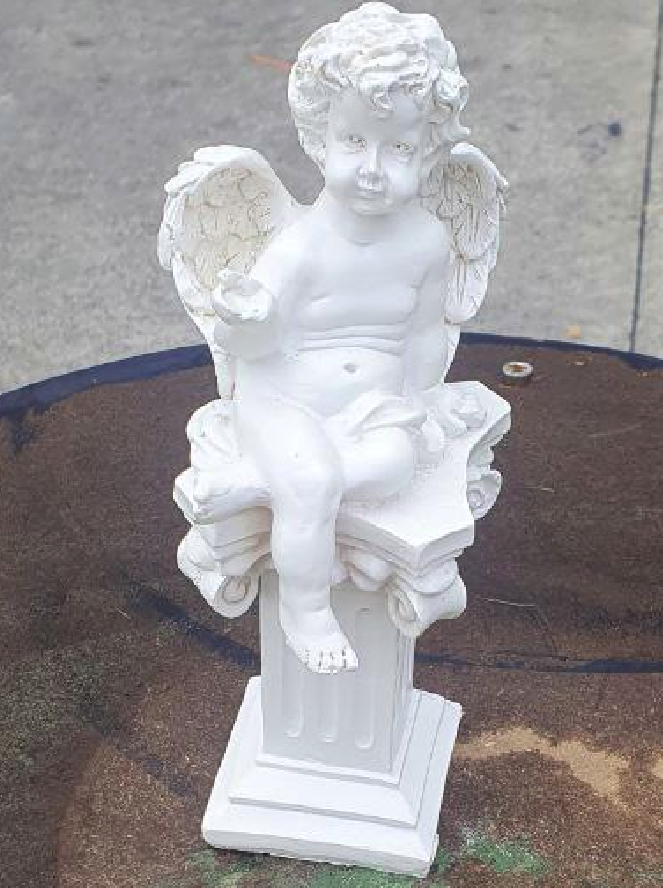
\includegraphics[keepaspectratio,width=0.35\textwidth]{angel}
\end{figure}

119 photos of it were collected, all around it and at three different heights. The 3D model was obtained with Zephyr after the following steps:
\begin{itemize}
\item Sparse point cloud generation, using the 'Human body' and 'High details' presets.
\item Dense point cloud generation, using the 'Human body' and 'High details' presets.
\item Mesh generation, using the 'Default' and 'High details' presets.
\item Textured mesh generation, using the 'Default' and 'High details' presets.
\end{itemize}

\begin{figure}[H]
\centering
\begin{minipage}{0.23\textwidth}
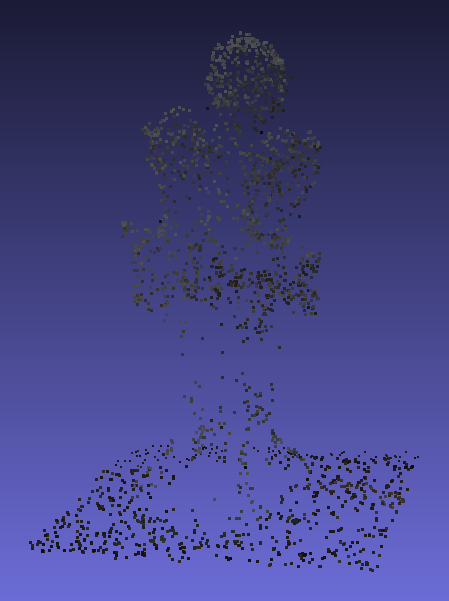
\includegraphics[keepaspectratio,width=0.9\textwidth]{angel_sparse}
\end{minipage}
\begin{minipage}{0.25\textwidth}
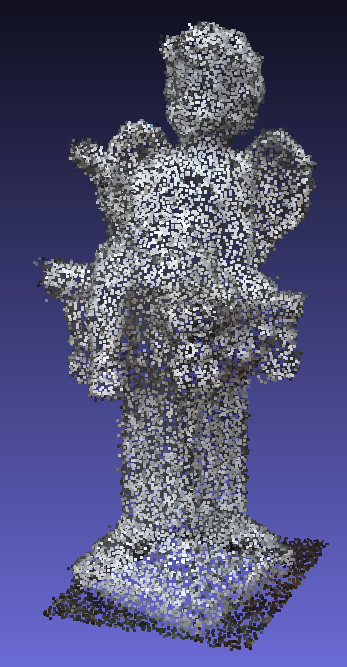
\includegraphics[keepaspectratio,width=0.9\textwidth]{angel_dense}
\end{minipage}
\begin{minipage}{0.25\textwidth}
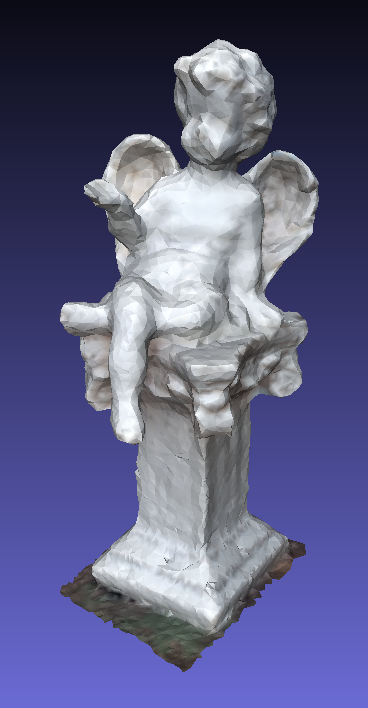
\includegraphics[keepaspectratio,width=0.9\textwidth]{angel_mesh}
\end{minipage}
\begin{minipage}{0.25\textwidth}
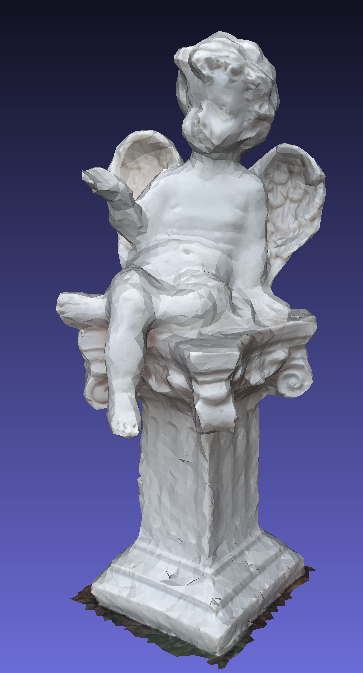
\includegraphics[keepaspectratio,width=0.9\textwidth]{angel_textured_mesh}
\end{minipage}
\caption{From left to right: sparse point cloud, dense point cloud, mesh and textured mesh.}
\end{figure}

\section{Assignment 2}

\subsection{Implement in MATLAB the trapezoidal trajectory taking into account the different constraints.}

The general expression for a trapezoidal velocity profile is:

\begin{equation*}
q(t)=\begin{cases}
q_i+\dot q_i(t-t_i)+\frac{\dot q_c-\dot q_i}{2t_a}(t-t_i)^2 & t_i\leq t\leq t_a+t_i\\
q_i+\dot q_i\frac{t_a}{2}+\dot q_c(t-t_i-\frac{t_a}{2})^2 & t_a+t_i\leq t\leq t_f-t_d\\
q_f-\dot q_f(t_f-t)-\frac{\dot q_c-\dot q_f}{2t_d}(t_f-t)^2 & t_f-t_d\leq t\leq t_f
\end{cases}
\end{equation*}

If the initial and final velocities are null, then $t_a=t_d=t_c$.

If $\dot q_i=\dot q_f=0$ then the possible constraints are:
\begin{itemize}
\item $t_c$:
\begin{equation*}
\ddot q_c = \frac{q_f-q_i}{t_ct_f-t_c^2}\;\;\;\;\dot q_c=\ddot q_ct_c
\end{equation*}
\item $\ddot q_c$:
\begin{equation*}
t_c=\frac{t_f}{2}-\frac{1}{2}\sqrt{\frac{t_f^2\ddot q_c-4(q_f-q_i)}{\ddot q_c}}\;\;\;\;\dot q_c=\ddot q_ct_c
\end{equation*}
\item $\dot q_c$:
\begin{equation*}
t_c=\frac{q_i-q_f+\dot q_ct_f}{\dot q_c}\;\;\;\;\ddot q_c = \frac{\dot q_c^2}{q_i-q_f+\dot q_ct_f}
\end{equation*}
\item $\ddot q_c,\dot q_c$:
\begin{equation*}
t_c=\frac{\dot q_c}{\ddot q_c}\;\;\;\;t_f=\frac{\dot q_c^2+\ddot q_c(q_f-q_i)}{\dot q_c\ddot q_c}
\end{equation*}
\end{itemize}

In all cases the feasibility condition is that $2t_c\leq t_f-t_i$.

If $\dot q_i,\dot q_f\neq 0$ the possible constraints are:

\begin{itemize}
\item $\ddot q_{c,max}$:
\begin{equation*}
\dot q_c = \frac{1}{2}(\dot q_i+\dot q_f+\ddot q_{c,max}\Delta T+\sqrt{\ddot q_{c,max}^2\Delta T^2-4\ddot q_{c,max}\Delta q+2\ddot q_{c,max}(\dot q_i+\dot q_f)\Delta T-(\dot q_i-\dot q_f)^2}\;\;\;\;\;t_a=\frac{\dot q_c-\dot q_i}{\ddot q_{c,max}}\;t_d=\frac{\dot q_c-\dot q_f}{\ddot q_{c,max}}
\end{equation*}

The trajectory is feasible when the argument of the square root is positive, and when the maximum acceleration satisfies:

\begin{equation*}
\ddot q_{c,max}\Delta q>\frac{\abs{\dot q_i^2-\dot q_f^2}}{2}\;\;\;\ddot q_{c,max}\geq\ddot q_{c,lim}=\frac{2\Delta q-(\dot q_i-\dot q_f)\Delta T+\sqrt{4\Delta q^2-4\Delta q(\dot q_i+\dot q_f)\Delta T+2(\dot q_i^2+\dot q_f^2)\Delta T^2}}{\Delta T^2}
\end{equation*}

when $\ddot q_{c,max}=\ddot q_{c,lim}$ there is no constant velocity phase.
\item $\ddot q_{max},\dot q_{max}$:
First we compute the condition:
\begin{equation*}
\ddot q_{c,max}\Delta q\gtreqless\dot q_{c,max}^2-\frac{\dot q_i^2+\dot q_f^2}{2}
\end{equation*}

If the above is $>$ then:

\begin{equation*}
\dot q_c=\dot q_{c,max}\;\;\;t_a=\frac{\dot q_{c,max}-\dot q_i}{\ddot q_{c,max}}\;\;\;t_d=\frac{\dot q_{c,max}-\dot q_f}{\ddot q_{c,max}}\;\;\;\Delta T=\frac{\Delta q\ddot q_{c,max}+\dot q_{c,max}^2}{\ddot q_{c,max}\dot q_{c,max}}
\end{equation*}

If the above is $\leq$ then:
\begin{equation*}
\dot q_c=\dot q_{c,lim}=\sqrt{\ddot q_{c,max}\Delta q+\frac{\dot q_i^2+\dot q_f^2}{2}}<\dot q_{c,max}\;\;\;t_a=\frac{\dot q_{c,lim}-\dot q_i}{\ddot q_{c,max}}\;\;\;t_d=\frac{\dot q_{c,lim}-\dot q_f}{\ddot q_{c,max}}
\end{equation*}
\end{itemize}

\begin{figure}
\begin{minipage}{0.333\textwidth}
\centering
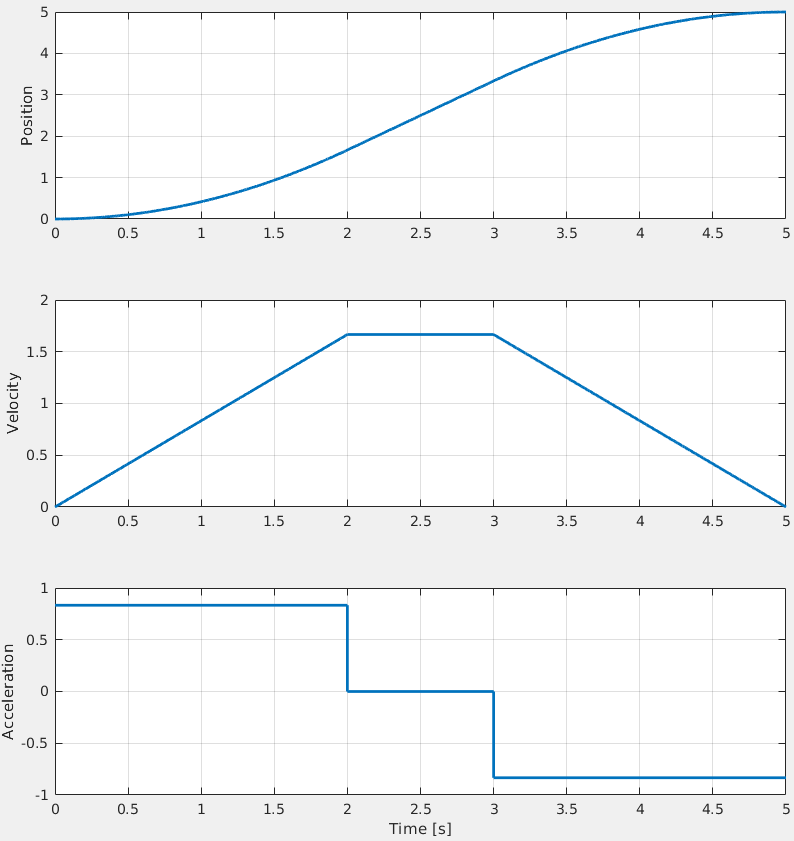
\includegraphics[keepaspectratio,width=\textwidth]{trap_1}
\caption{$t_c=2s$}
\label{fig:trap_1}
\end{minipage}
\begin{minipage}{0.333\textwidth}
\centering
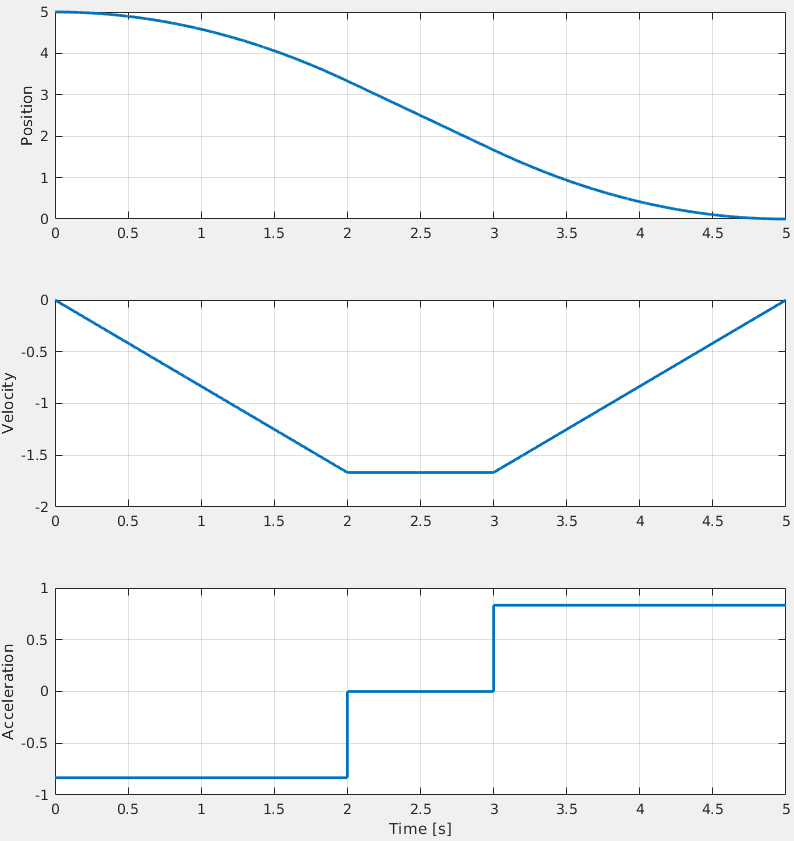
\includegraphics[keepaspectratio,width=\textwidth]{trap_2}
\caption{$t_c=2s, q_i>q_f$}
\label{fig:trap_2}
\end{minipage}
\begin{minipage}{0.333\textwidth}
\centering
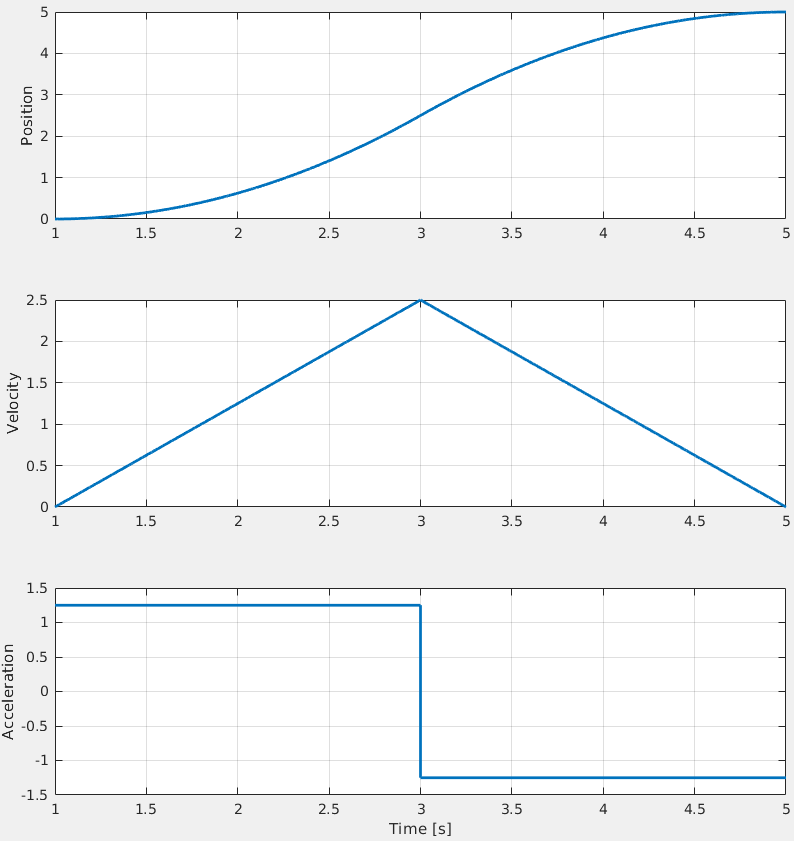
\includegraphics[keepaspectratio,width=\textwidth]{trap_3}
\caption{$t_c=2s, t_i\neq 0$}
\label{fig:trap_3}
\end{minipage}
\end{figure}

\begin{figure}
\begin{minipage}{0.5\textwidth}
\centering
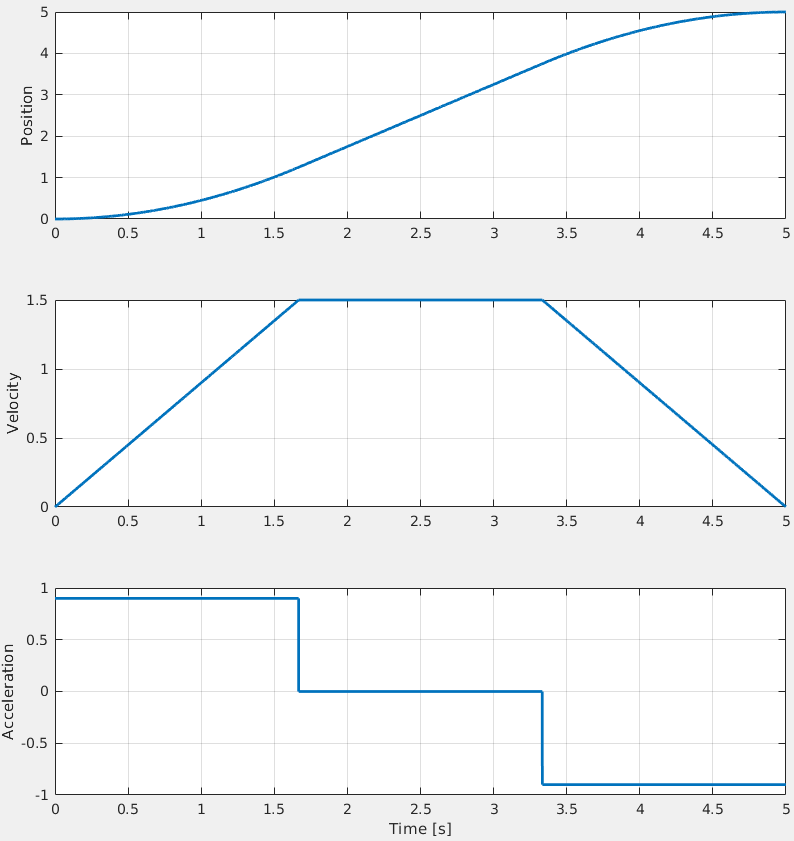
\includegraphics[keepaspectratio,width=\textwidth]{trap_5}
\caption{$v_c=1.5$}
\label{fig:trap_5}
\end{minipage}
\begin{minipage}{0.5\textwidth}
\centering
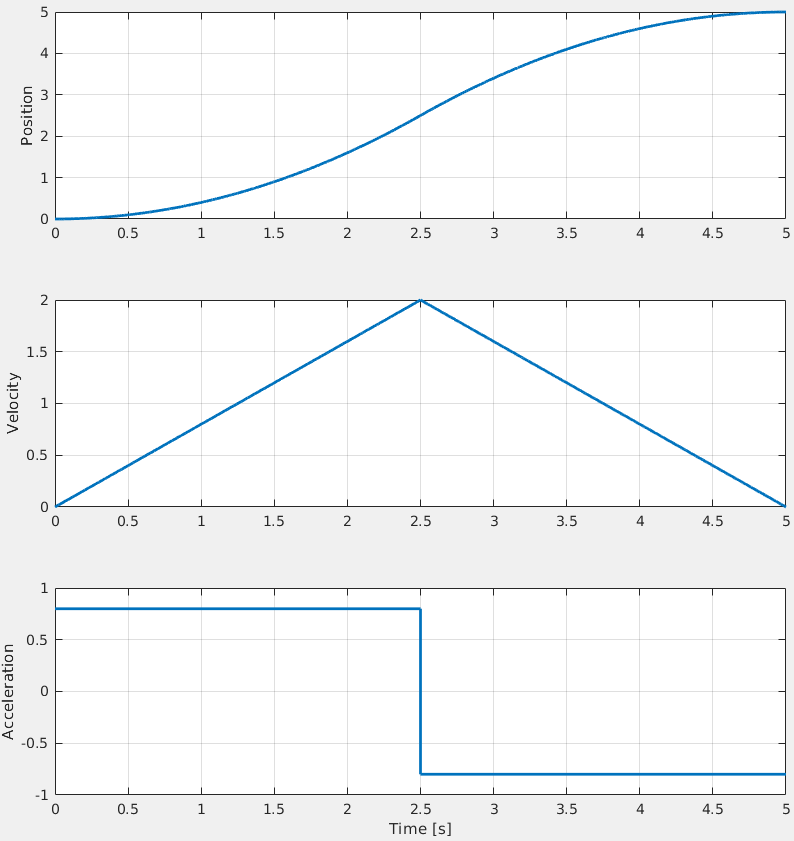
\includegraphics[keepaspectratio,width=\textwidth]{trap_4}
\caption{$v_c=v_{c,lim}=2$}
\label{fig:trap_4}
\end{minipage}
\end{figure}

\begin{figure}
\begin{minipage}{0.5\textwidth}
\centering
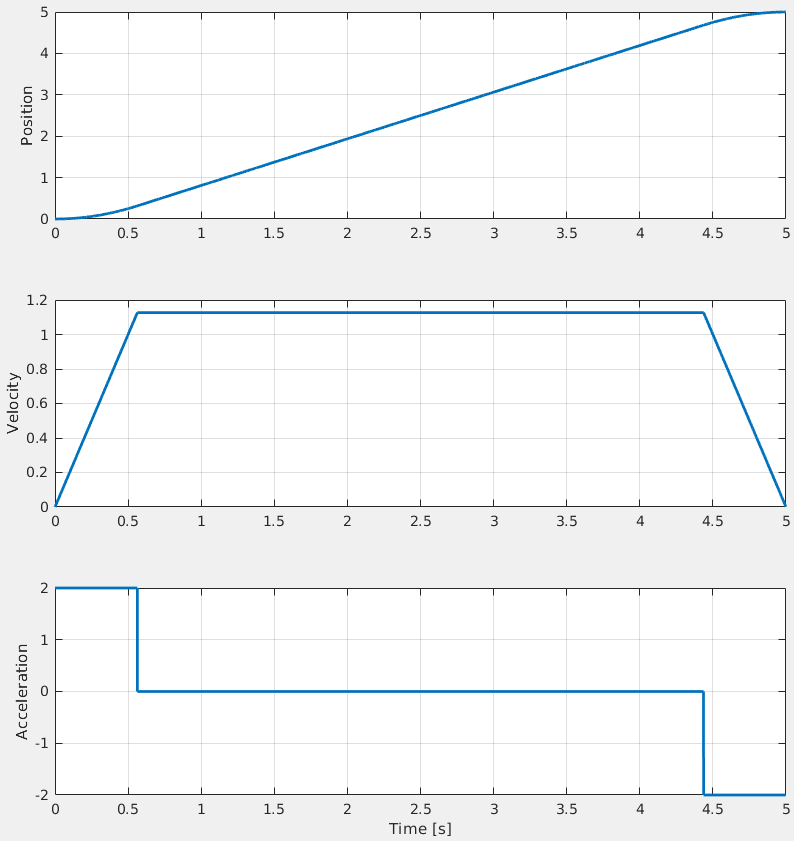
\includegraphics[keepaspectratio,width=\textwidth]{trap_6}
\caption{$a_c=2$}
\label{fig:trap_6}
\end{minipage}
\begin{minipage}{0.5\textwidth}
\centering
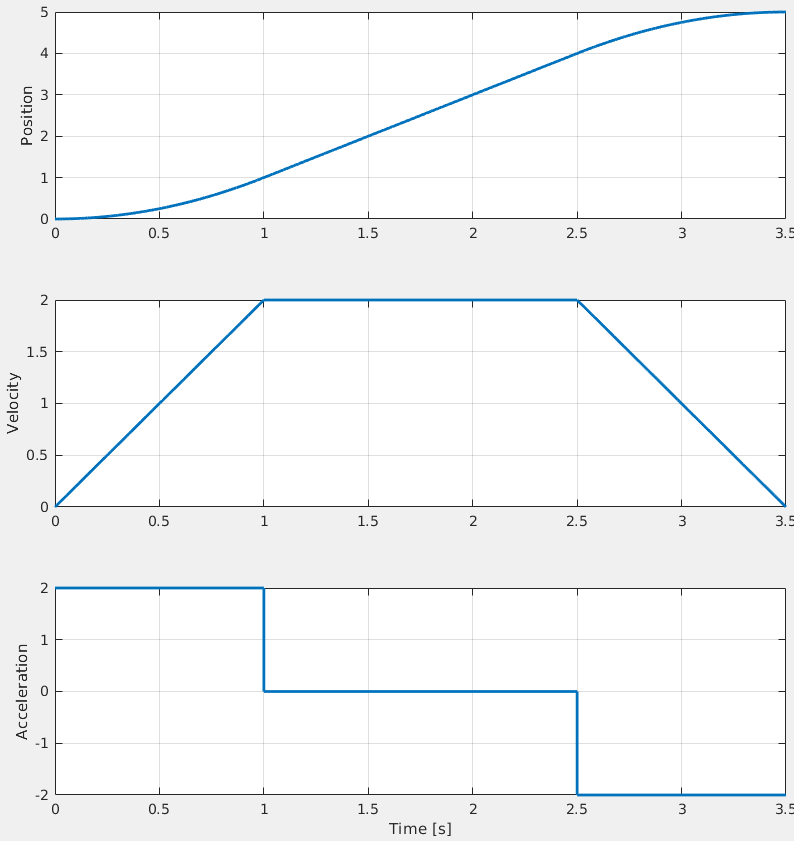
\includegraphics[keepaspectratio,width=\textwidth]{trap_7}
\caption{$a_c,v_c=2$}
\label{fig:trap_7}
\end{minipage}
\end{figure}

\begin{figure}
\begin{minipage}{0.5\textwidth}
\centering
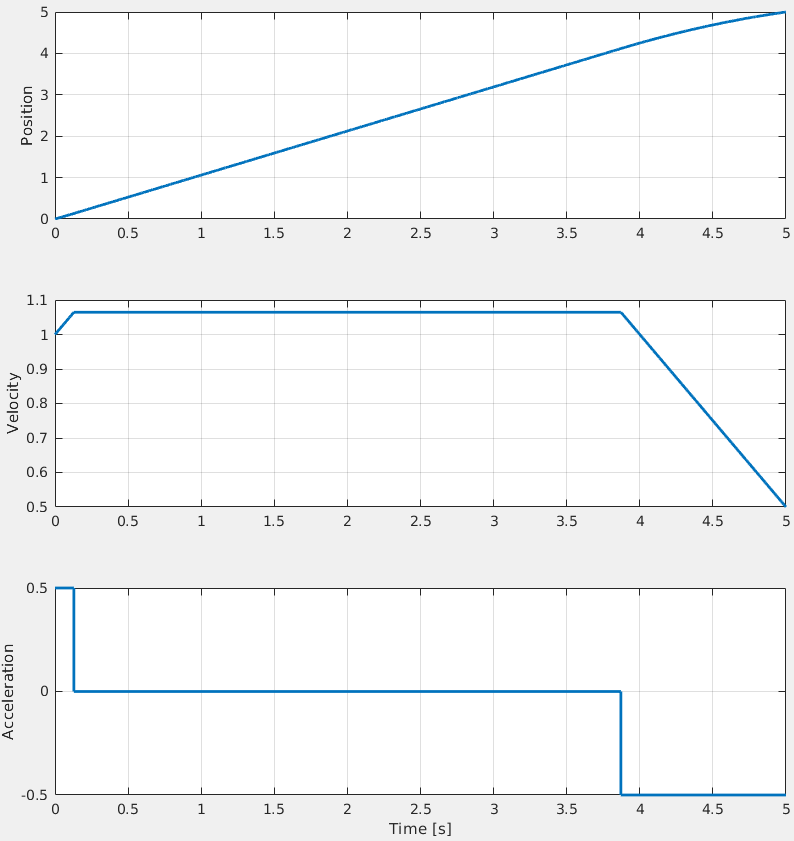
\includegraphics[keepaspectratio,width=\textwidth]{trap_8}
\caption{$\dot q_i=1,\dot q_f=0.5,\ddot q_{max}=0.5$}
\label{fig:trap_8}
\end{minipage}
\begin{minipage}{0.5\textwidth}
\centering
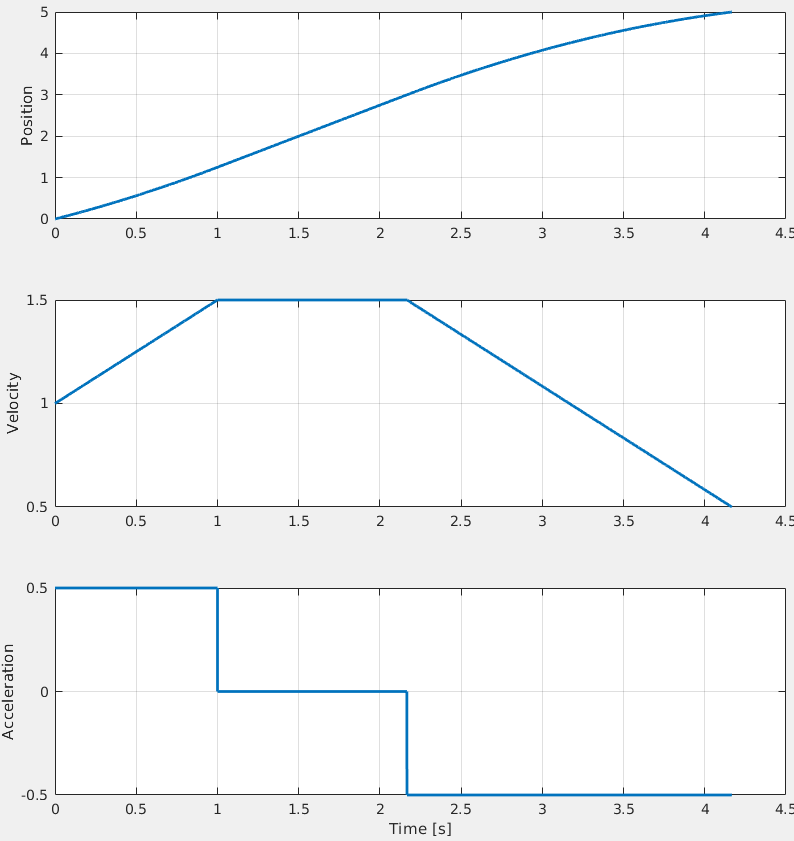
\includegraphics[keepaspectratio,width=\textwidth]{trap_9}
\caption{$\dot q_i=1,\dot q_f=0.5,\dot q_{max}=1.5,\ddot q_{max}=0.5$}
\label{fig:trap_9}
\end{minipage}
\end{figure}

To generate a multipoint trajectory we simply repeat the computation for each consecutive point pair. To improve the resulting velocity and acceleration profiles we can apply an heuristic to assign velocities to each waypoint, so that a less jagged profile is obtained:

\begin{align*}
\dot q(t_i)&=\dot q_i\\
\dot q(t_k)&=\begin{cases}
0 & \text{if }sign(\Delta Q_k)\neq sign(\Delta Q_{k+1})\\
sign(\Delta Q_k)\dot q_{max}& \text{if }sign(\Delta Q_k)= sign(\Delta Q_{k+1})\\
\end{cases}\\
\dot q(t_f)&=\dot q_f
\end{align*}

\begin{figure}
\begin{minipage}{0.5\textwidth}
\centering
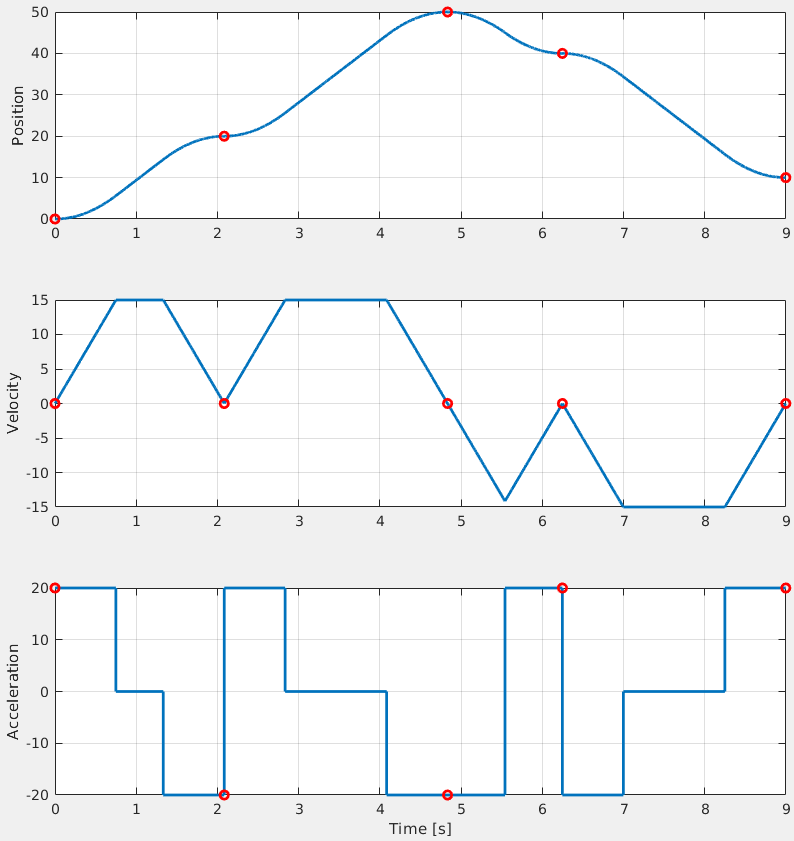
\includegraphics[keepaspectratio,width=\textwidth]{trap_10}
\caption{Multipoint trajectory without velocity heuristic}
\label{fig:trap_10}
\end{minipage}
\begin{minipage}{0.5\textwidth}
\centering
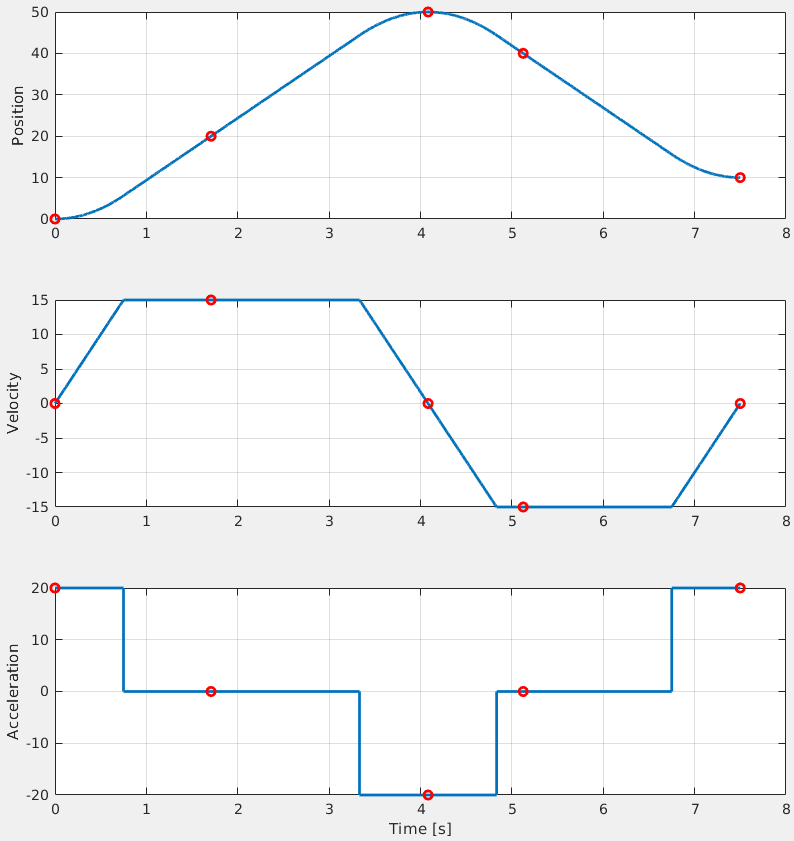
\includegraphics[keepaspectratio,width=\textwidth]{trap_11}
\caption{Multipoint trajectory with velocity heuristic}
\label{fig:trap_11}
\end{minipage}
\end{figure}

\section{Assignment 3}
\subsection{Interpolating polynomials with computed velocities at path points and imposed velocity at initial/final points.}

To implement multipoint trajectories we concatenate cubic splines. The interpolating trajectory is then:

\begin{equation*}
q(t)\coloneqq\{\Pi_k(t),t\in[t_k,t_{k+1}],k=0,\dots,n-1\}
\end{equation*}

where:

\begin{equation*}
\Pi(t)=a_3^k(t-t_k)^3+a_2^k(t-t_k)^2+a_1^k(t-t_k)+a_0^k
\end{equation*}

Fixing velocities on all path points yields:

\begin{equation*}
\begin{cases}
a_0^k&=q_k\\
a_1^k&=\dot q_k\\
a_2^k&=\frac{1}{T_k}\left(\frac{3(q_{k+1}-q_k)}{T_k}-2\dot q_k-\dot q_{k+1}\right)\\
a_3^k&=\frac{1}{T_k^2}\left(\frac{^2(q_{k}-q_{k+1})}{T_k}+\dot q_k+\dot q_{k+1}\right)\\
\end{cases}
\end{equation*}

where $T_k=t_{k+1}-t_k$.

\begin{figure}[h]
\centering
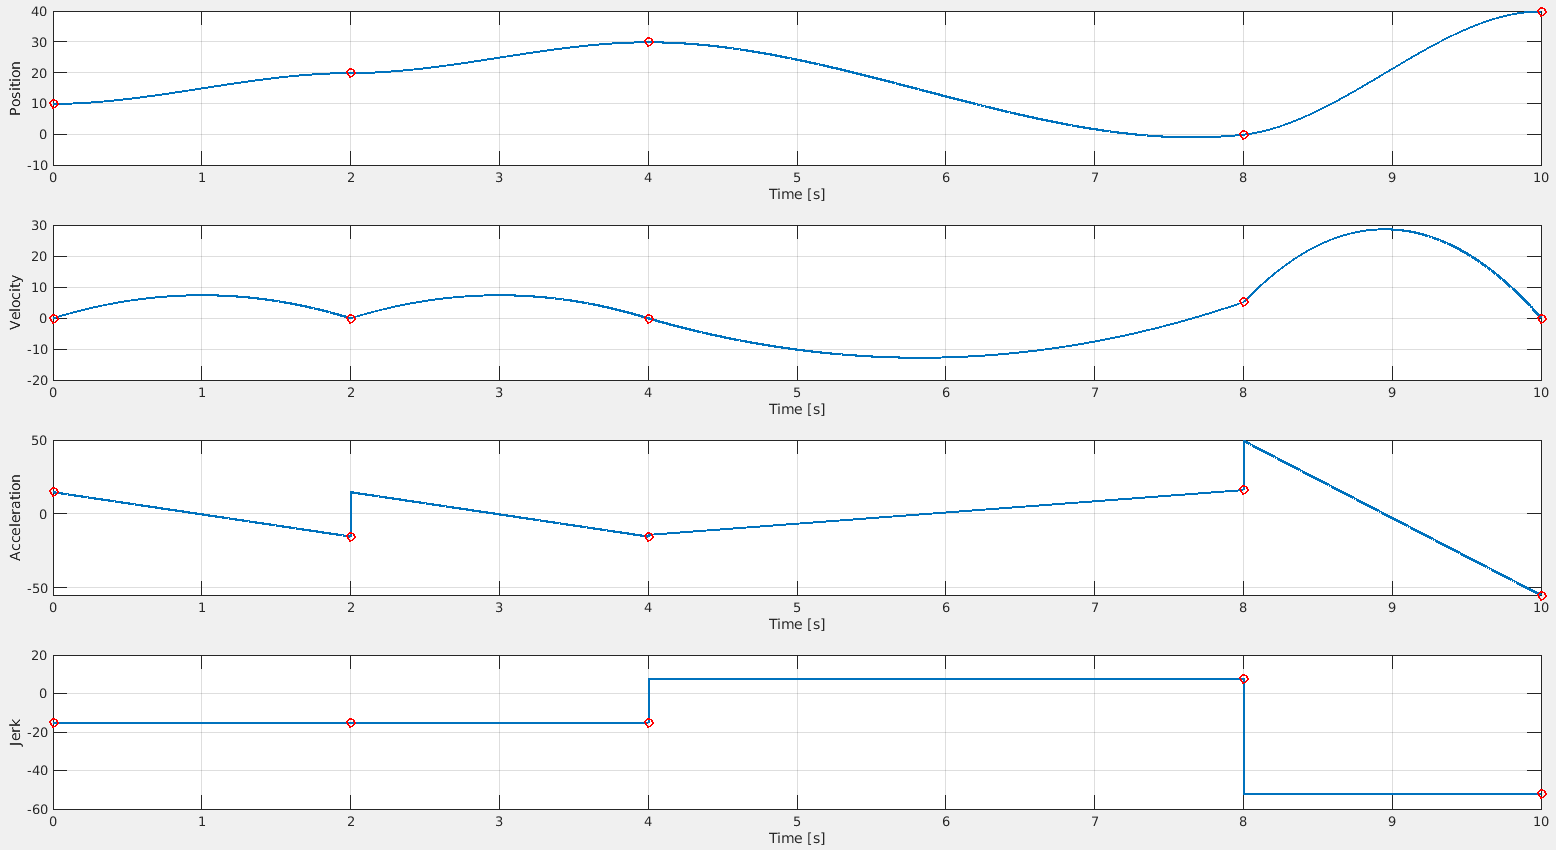
\includegraphics[keepaspectratio,width=0.7\textwidth]{cubic_1}
\caption{Trajectory through $q_k=\begin{bmatrix}
10 & 20 & 0 & 30 & 40
\end{bmatrix}$ at times $t_k=\begin{bmatrix}
0 & 2 & 4 & 8 & 10
\end{bmatrix}$ with \\velocities $\dot q_k=\begin{bmatrix}
0 & 0 & 0 & 5.2 & 0
\end{bmatrix}$}
\end{figure}

\newpage

\subsection{Interpolating polynomials with continuous accelerations at path points and imposed velocity at initial/final points (+ Thomas algorithm)}

Path point velocities are not generally known. We can estimate them with Euler's approximation:

\begin{equation*}
v_k = \frac{q_k-q_{k-1}}{t_k-t_{k-1}}\implies\begin{cases}
\dot q(t_0)&=\dot q_0\\
\dot q(t_k)&=\begin{cases}
0 & \text{if }sign(\Delta Q_k)\neq sign(v_{k+1})\\
\frac{v_k+v_{k+1}}{2} &  \text{if }sign(v_k) =  sign(v_{k+1})\\
\end{cases}\\
\dot q(t_n) &= \dot q_n
\end{cases}
\end{equation*}

Imposing acceleration continuity at path points results in the definition of a linear system $A\dot q=c$, where $A$ is a tridiagonal matrix. Thanks to this property the system can be solved for $\dot q$ efficiently using Thomas' algorithm. Given:

\begin{equation*}
\begin{bmatrix}
b_1 & c_1 & 0 & \dots\\
a_2 & b_2 & c_2 & 0 & \dots\\
0 & \ddots & \ddots & \ddots & 0 & \dots\\
& 0 & a_k & b_k & c_k & 0 & \dots\\
& & 0 & \ddots & \ddots & \ddots & 0 \\
& & & 0 & a_{n-1} & b_{n-1} & c_{n-1}\\
& & & & 0 & a_n & b_n
\end{bmatrix}\begin{bmatrix}
\dot q_1\\\vdots\\\dot  q_k\\\vdots \\ \dot q_n
\end{bmatrix}=\begin{bmatrix}
d_1\\\vdots\\ d_k\\\vdots \\ d_n
\end{bmatrix}
\end{equation*}

Thomas' algorithm is as follows:

\begin{minipage}{0.5\textwidth}
Forward elimination:
\begin{center}
\begin{algorithmic}
    \For{$k=2:1:n$} 
        \State {$m$ $\gets$ {$\frac{a_k}{b_{k-1}}$}}
        \State{$b_k$ $\gets$ {$b_k-mc_{k-1}$}}
        \State{$d_k$ $\gets$ {$d_k-md_{k-1}$}}
    \EndFor
\end{algorithmic}
\end{center}
\end{minipage}
\begin{minipage}{0.5\textwidth}
Backward substitution:
\begin{center}
\begin{algorithmic}
\State{$x_n$ $\gets$ $\frac{d_n}{b_n}$}
    \For{$k=2:1:n$} 
        \State{$x_k$ $\gets$ {$\frac{d_k-c_kx_{k+1}}{b_k}$}}
    \EndFor
\end{algorithmic}
\end{center}
\end{minipage}


\begin{figure}[h]
\begin{minipage}{0.5\textwidth}
\centering
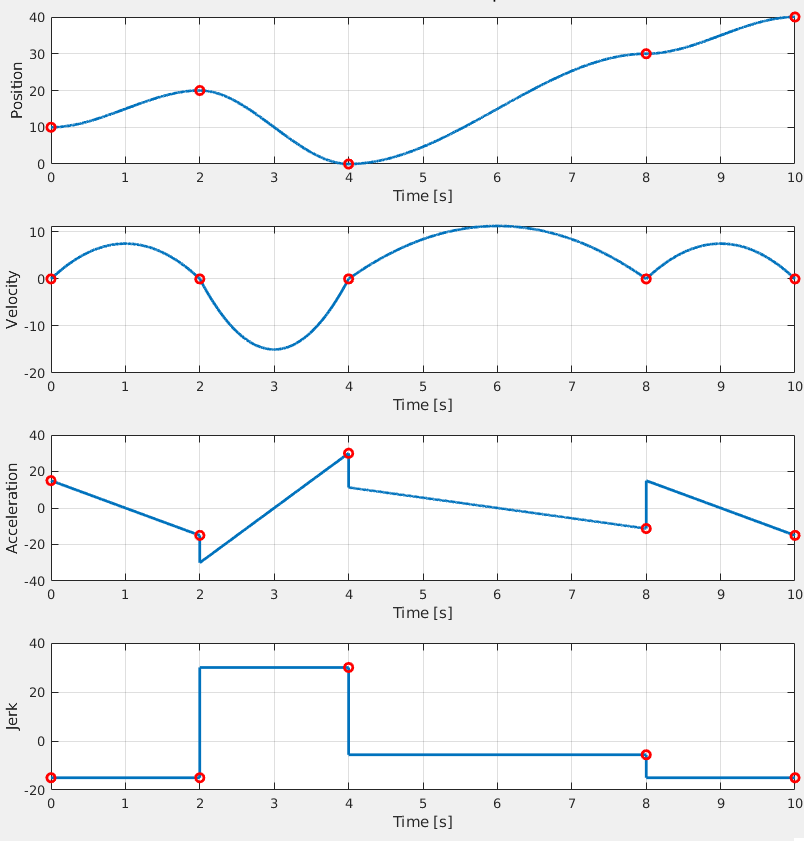
\includegraphics[keepaspectratio,width=\textwidth]{cubic_2}
\caption{Trajectory interpolation with Euler's approximation.}
\end{minipage}
\begin{minipage}{0.5\textwidth}
\centering
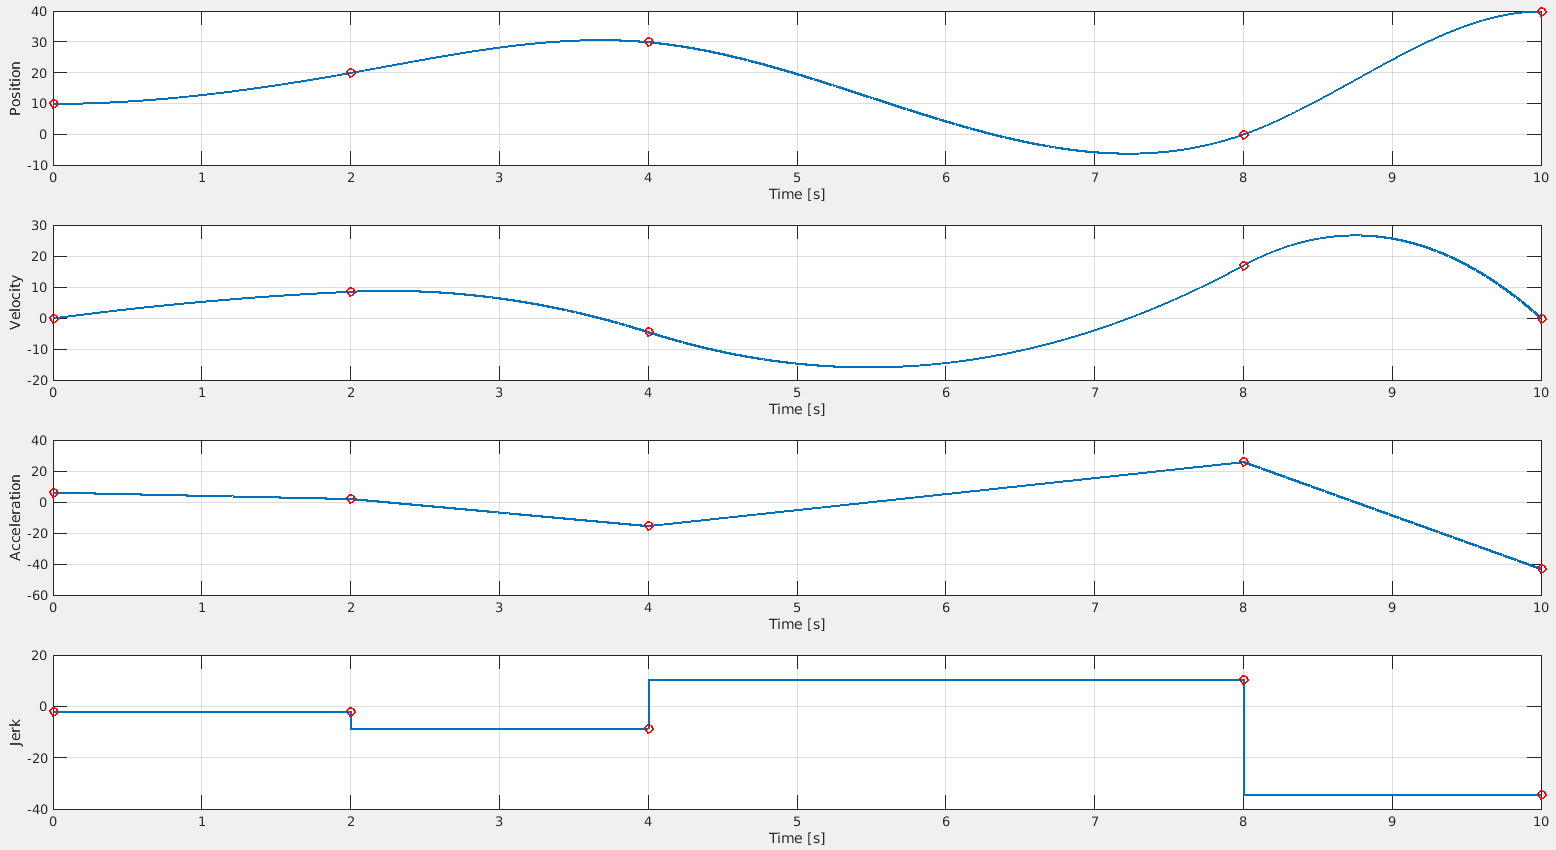
\includegraphics[keepaspectratio,width=\textwidth]{cubic_3}
\caption{Trajectory interpolation with continuous accelerations.}
\end{minipage}
\end{figure}

\section{Assignment 4}

\subsection{Image analysis using morphological operators}

2D image analysis can be carried out with the use of morphological operators. Image closing and opening let us remove the background of pictures and isolate the objects within them. More complex operations can then be carried out, inferring for example geometric information on the shapes produced.

Classification used the 'Circularity' property to distinguish between coins and USB stick, as well as the 'MajorAxis' and 'MinorAxis' properties, which were averaged to compute the radius of the coins to detect which was smaller and which was bigger.

\subsubsection{Example 1}

Background removed by opening with a structuring element in the shape of a disk of size 65. Shapes improved by image closing with a structuring element in the shape of a disk of size 25 and by filling holes. Noise removed after image binarization with area opening, removing all shapes with fewer than 50 pixels.

Classification used the 'Circularity' property to distinguish between coins and USB stick, as well as the 'MajorAxis' and 'MinorAxis' properties, which were averaged to compute the radius of the coins to detect which was smaller and which was bigger.

\begin{figure}[h]
\centering
\begin{minipage}{0.45\textwidth}
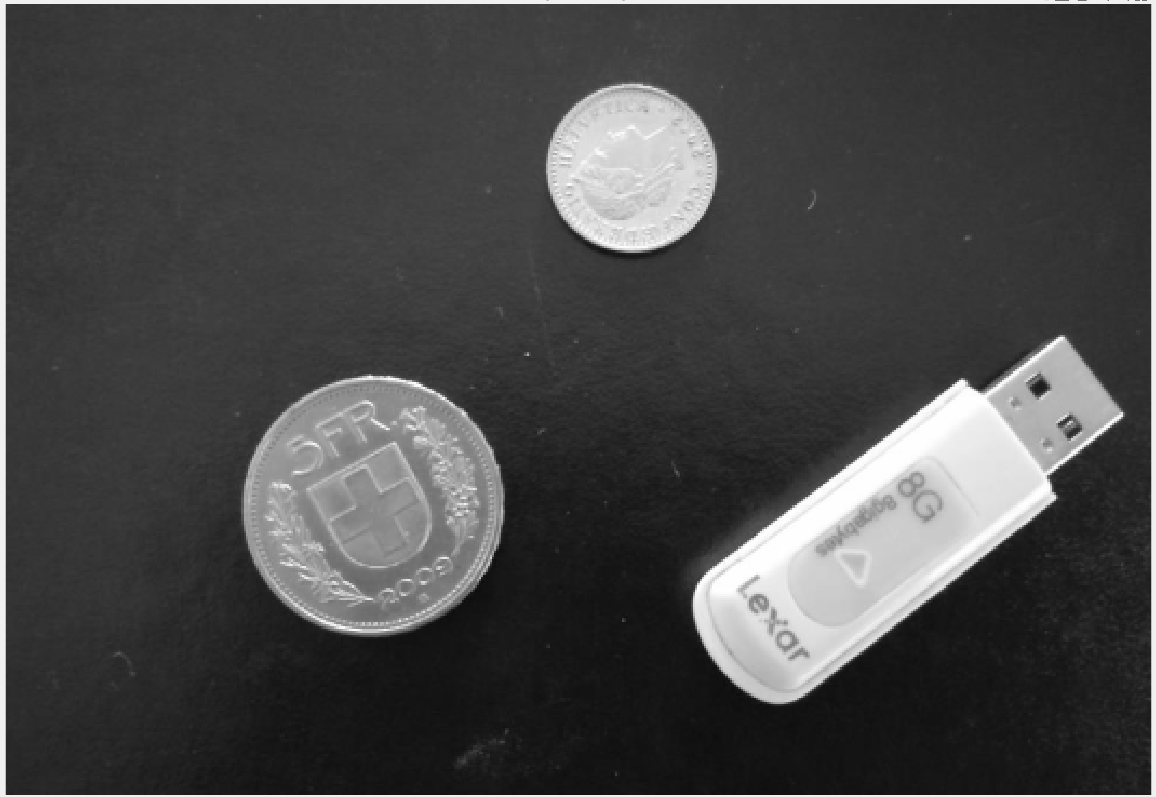
\includegraphics[keepaspectratio,width=0.9\textwidth]{4_coins_original}
\end{minipage}
\begin{minipage}{0.45\textwidth}

\includegraphics[keepaspectratio,width=0.9\textwidth]{4_coins_shapes}
\end{minipage}
\caption{Original image (left) vs extracted shapes (right).}
\end{figure}
\begin{figure}[h]
\centering
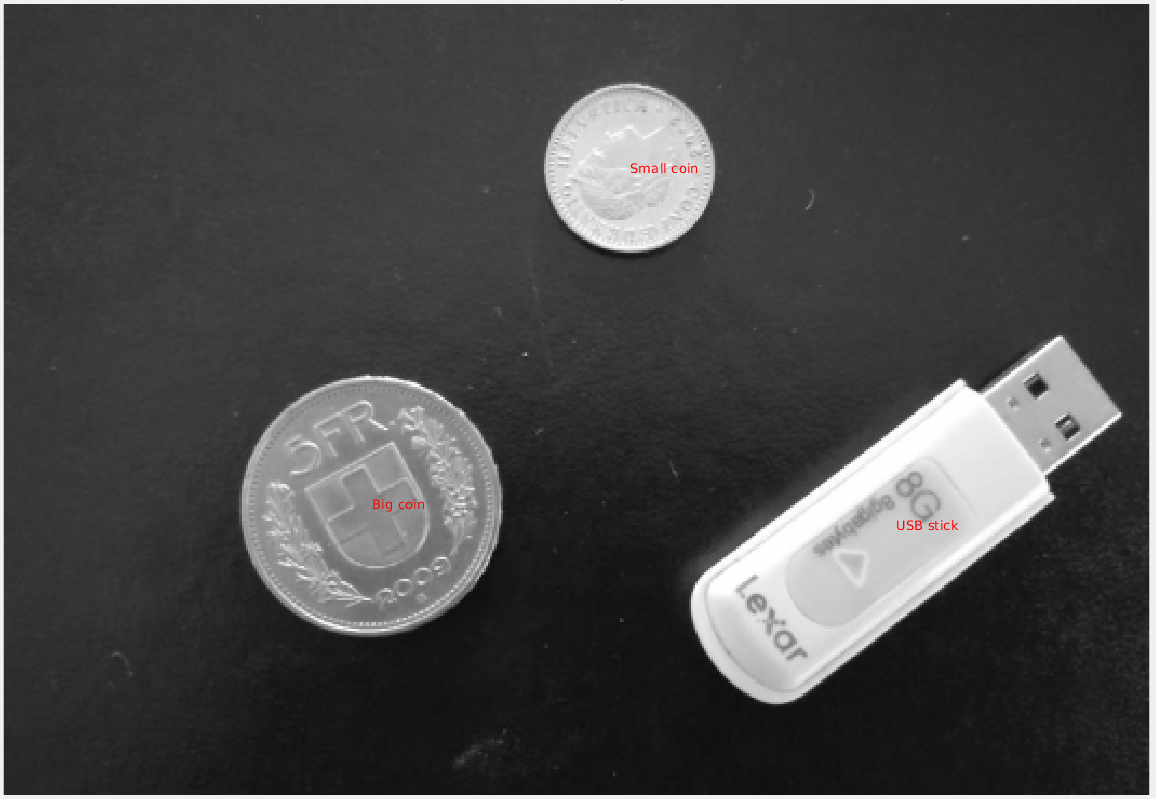
\includegraphics[keepaspectratio,width=0.5\textwidth]{4_coins_labels}
\caption{Labeled image.}
\end{figure}

\newpage

\subsubsection{Example 2}

Background removed by opening with a structuring element in the shape of a disk of size 65. Shapes improved by image closing with a structuring element in the shape of a disk of size 25 and by filling holes. Noise removed after image binarization with area opening, removing all shapes with fewer than 50 pixels.

Classification used the 'Circularity' property to distinguish between washers and bolts. The 'MajorAxis' and 'MinorAxis' properties were averaged to compute the outer radius of the washers, on which a quintic polynomial was fit to determine the relation with the actual inner diameter. For the bolts, the 'Orientation' property was used to align the shapes vertically, so that the bottom part of them, which contains the threaded part, could be extracted. On the extracted shapes, the 'MajorAxis' and 'MinorAxis' properties were extracted and used to fit cubic polynomials to determine, respectively, the bolt length and diameter.

\begin{figure}[h]
\centering
\begin{minipage}{0.3\textwidth}
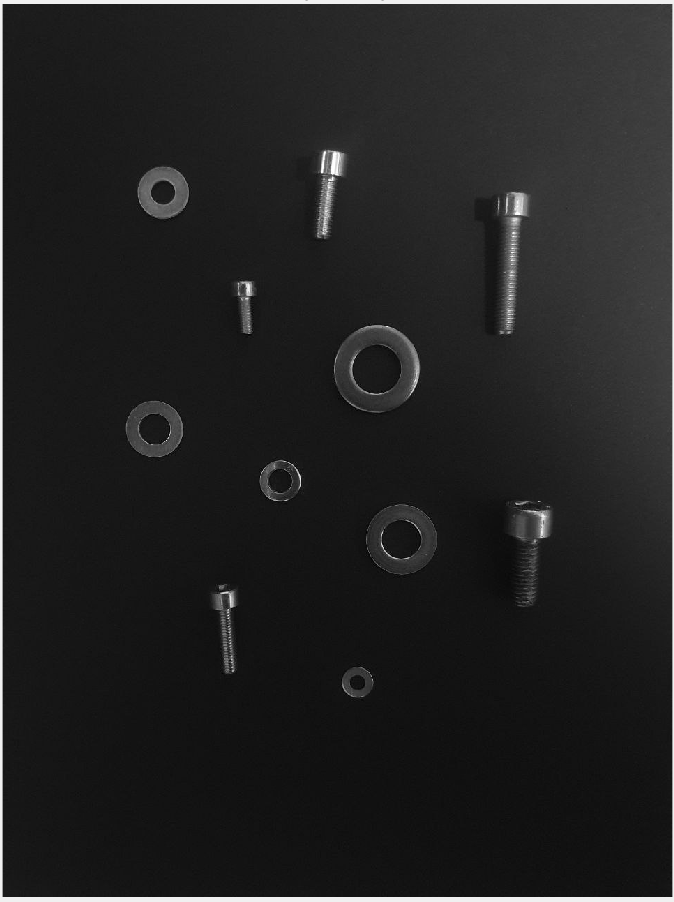
\includegraphics[keepaspectratio,width=0.9\textwidth]{4_nuts_original}
\end{minipage}
\begin{minipage}{0.3\textwidth}
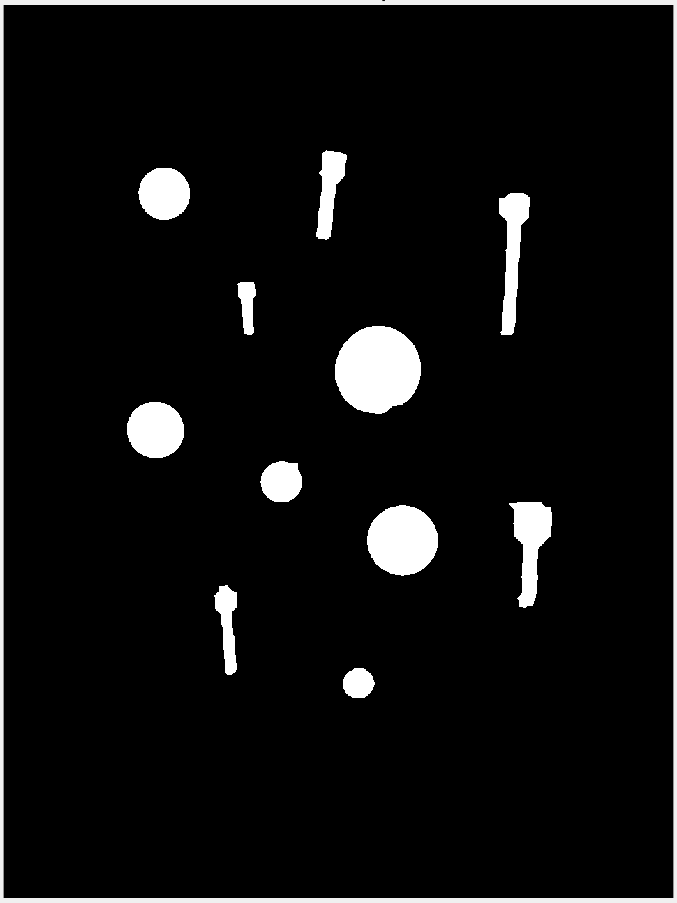
\includegraphics[keepaspectratio,width=0.9\textwidth]{4_nuts_shapes}
\end{minipage}
\begin{minipage}{0.3\textwidth}
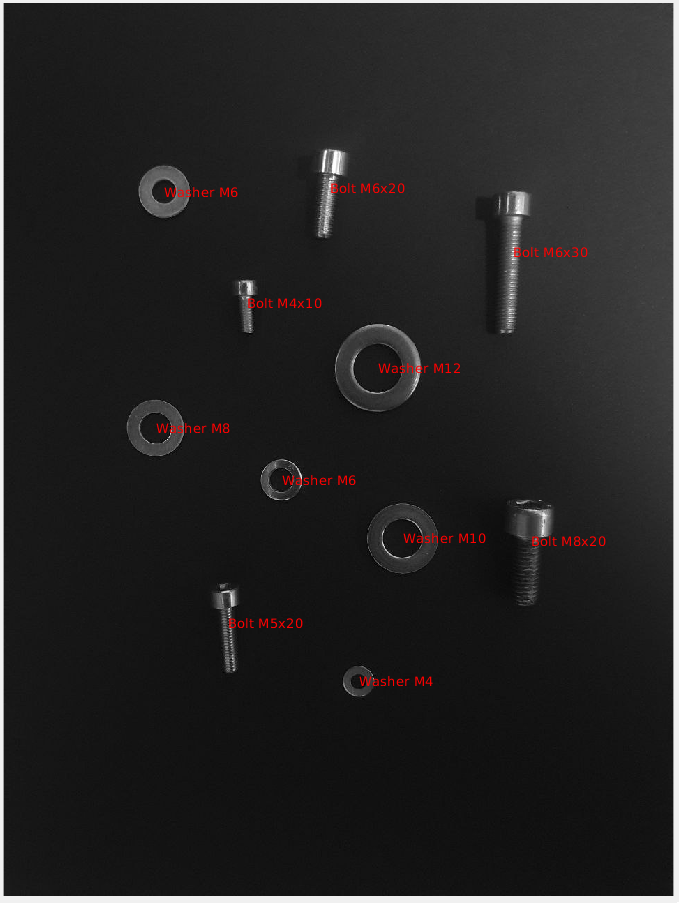
\includegraphics[keepaspectratio,width=0.9\textwidth]{4_nuts_labels}
\end{minipage}
\caption{Original image (left) vs extracted shapes (middle) vs labels (right).}
\end{figure}

\section{Assignment 5}

\subsection{Compute the 3D trajectory (position, velocity, acceleration and jerk) in the picture as
a combination of linear and circular motion primitives and compare it with the
trajectory obtained using one of the multi-point methods.}

\begin{figure}[h]
\centering
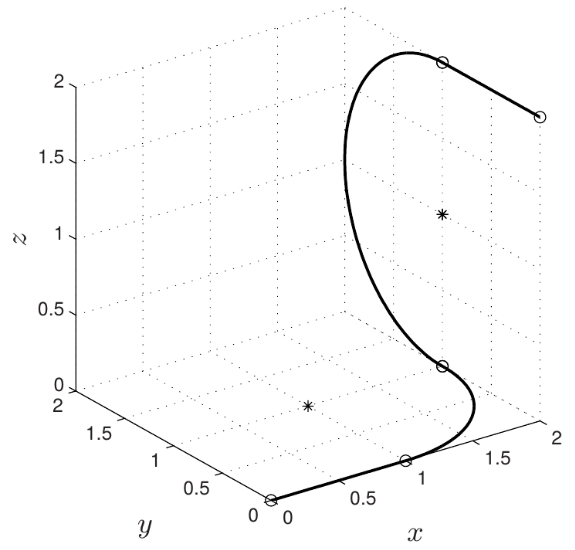
\includegraphics[keepaspectratio,width=0.35\textwidth]{3Dtraj_ref}
\caption{3D trajectory - reference.}
\end{figure}

Operational space trajectories can be computed by composing multiple motion primitives. The motion primitives used here are:

\begin{itemize}
\item Rectilinear path:
\begin{equation*}
p(u)=p_i+u(p_f-p_i)\;\;\;\;\;u\in[0,1]
\end{equation*}
\item Circular path:
\begin{equation*}
p(u)=c+Rp'(u)=c+R\begin{bmatrix}
\rho\cos(u)\\\rho\sin(u)\\
0
\end{bmatrix}=c+\begin{bmatrix}
(P-c)' & e_3'\cross(P-c)' & e_3'
\end{bmatrix}\begin{bmatrix}
\rho\cos(u)\\\rho\sin(u)\\
0
\end{bmatrix}\;\;\;\;\;u\in[0,\theta]
\end{equation*}

where $c$ is the position of the center of the circular path, $P$ is the position of the starting point on the circle and $e_3=\begin{bmatrix}
0 & 0 & 1
\end{bmatrix}$.
\end{itemize}

For comparison, a 3D trajectory is computed by computing the smoothing cubic splines along the three directions. The smoothing spline trajectory is also computed with added waypoints to improve the tracking of the position.

\begin{figure}[H]
\centering
\includegraphics[keepaspectratio,width=0.4\textwidth]{3Dtraj}
\caption{3D trajectory - motion primitives vs smoothing splines ($w_k=\infty\forall k$, $\mu=1$).}
\end{figure}

\begin{figure}[h]
\centering
\includegraphics[keepaspectratio,width=0.6\textwidth]{3Dtraj_pos}
\caption{3D trajectory - Position comparison.}
\end{figure}

\begin{figure}[h]
\centering
\includegraphics[keepaspectratio,width=0.9\textwidth]{3Dtraj_profiles}
\caption{3D trajectory - Velocity, acceleration, jerk comparison.}
\end{figure}

\section{Assignment 6}

\subsection{Pose reconstruction pipeline}

\section{Assignment 7}

\subsection{Plan the pick-and-place task for the UR5 robot in ROS for four cubes using three different orientations for the end-effector.}

The pick-and-place task is divided into two phases: scanning and pick-and-place.

The scanning consists of a composition of rectilinear and circular motion primitives that make sure that the camera mounted on the end-effector of the robot covers the whole workspace, detecting all cubes and their destination.

\begin{figure}[h]
\centering
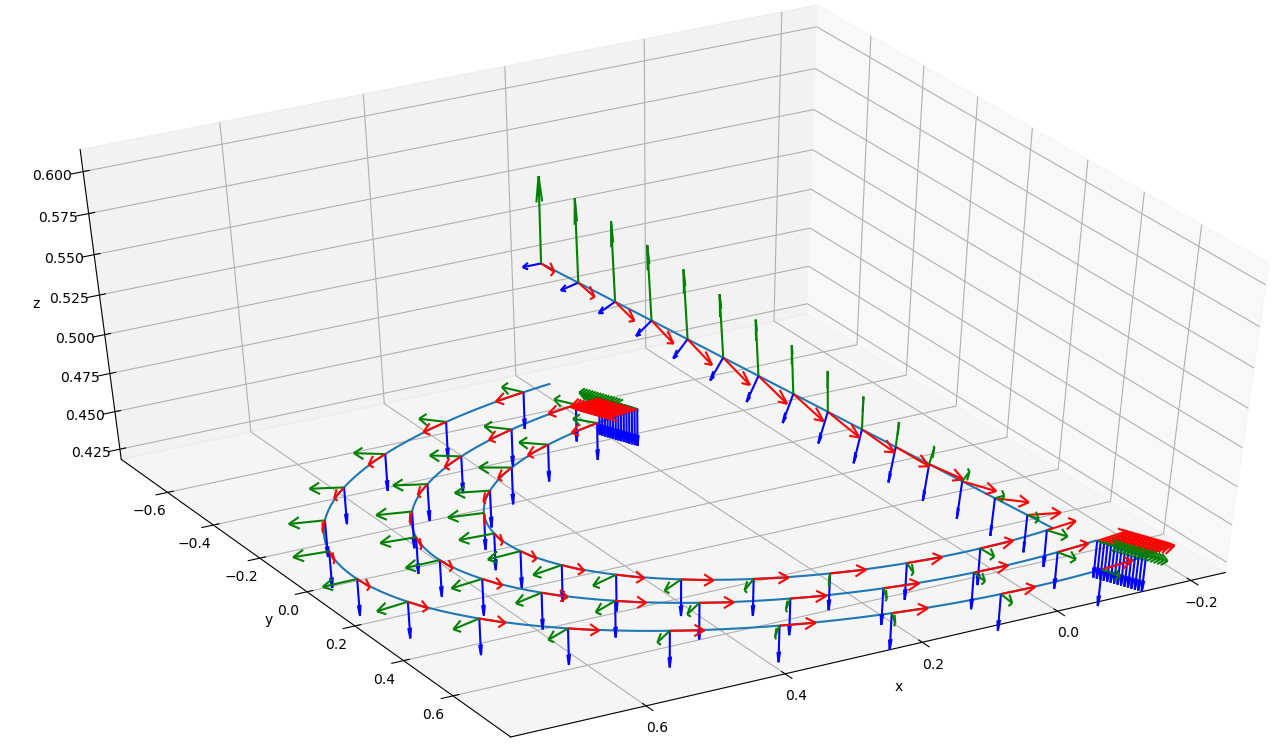
\includegraphics[keepaspectratio,width=0.9\textwidth]{scanning}
\caption{End-effector path and associated Frenet frames for the scanning phase.}
\end{figure}

\begin{figure}[h]
\centering
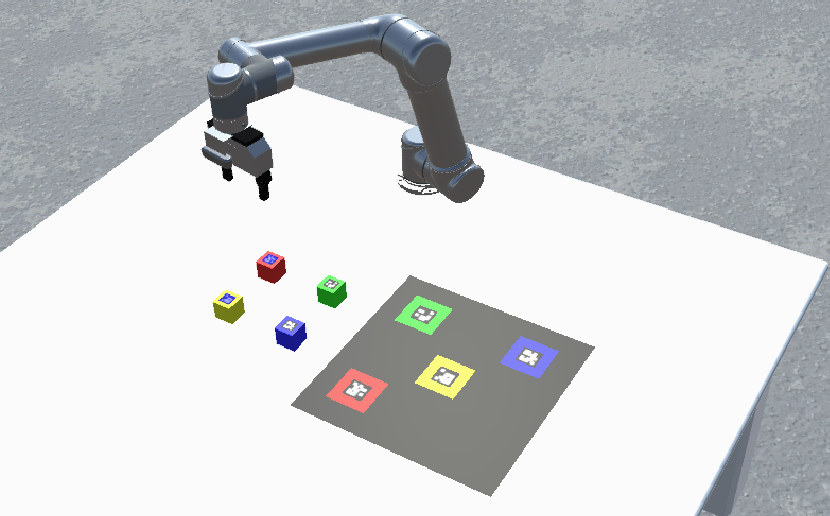
\includegraphics[keepaspectratio,width=0.6\textwidth]{scanning_sim}
\caption{Scanning task in Unity. The highlighted ARUCO markers are the ones currently detected by the end-effector camera.}
\end{figure}

\newpage

After the cubes and their destinations have been found, the pick-and-place phase is carried out as follows:

\begin{itemize}
\item Move linearly in Cartesian space towards the cube location.
\item Lower the end-effector onto the cube, close the gripper and then raise the end-effector back up.
\item Move linearly to the home position.
\item Move linearly to the destination, open the gripper and then raise the end-effector back up.
\item Move linearly to the home position.
\end{itemize}

\begin{figure}[h]
\centering
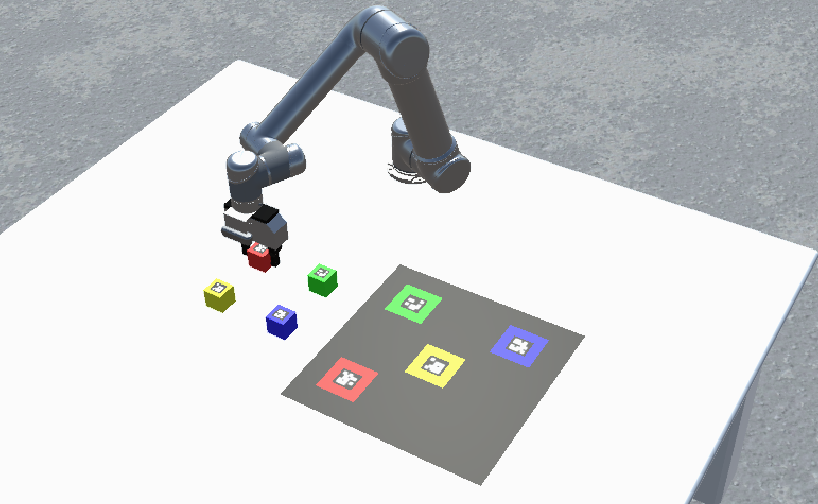
\includegraphics[keepaspectratio,width=0.4\textwidth]{pick}
\caption{Pick}
\end{figure}
\begin{figure}[h]
\centering
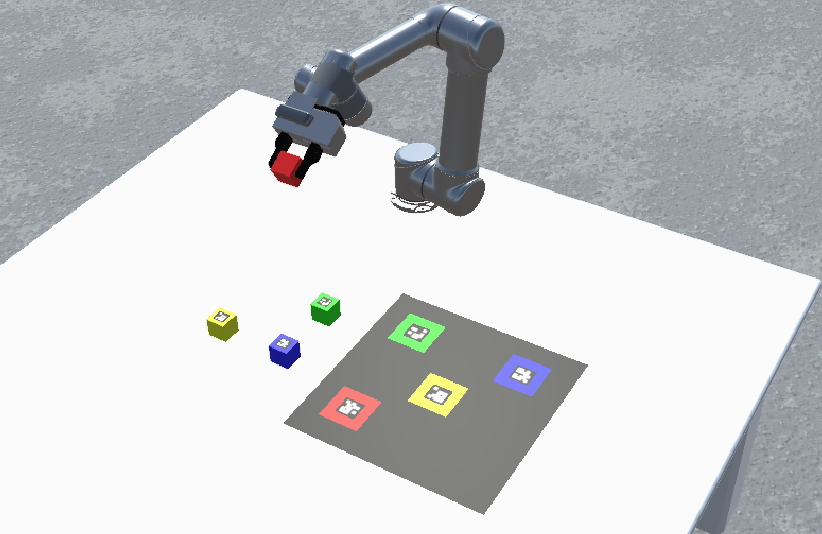
\includegraphics[keepaspectratio,width=0.4\textwidth]{home_w_cube}
\caption{Homing}
\end{figure}
\begin{figure}[h]
\centering
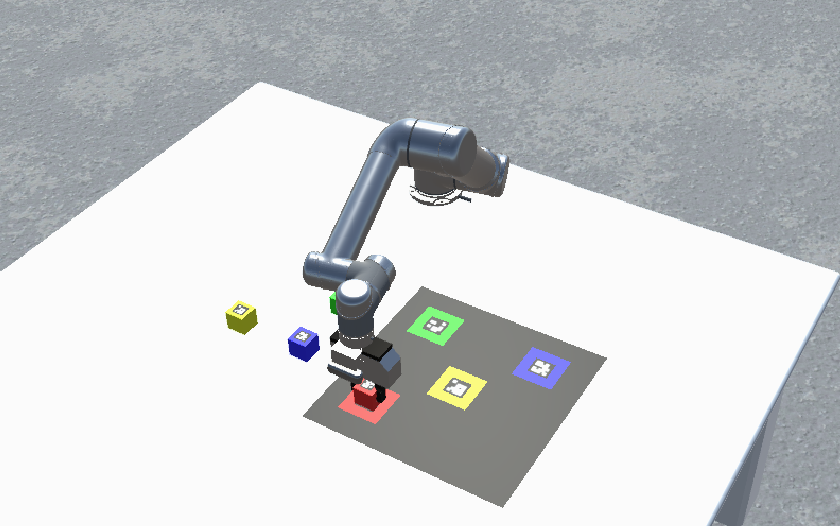
\includegraphics[keepaspectratio,width=0.4\textwidth]{place}
\caption{Place}
\end{figure}

\chapter{Vision}

\section{Assignment 1}

\subsection{3D model creation using Zephyr}

The object chosen for the assignment was a plastic statue of an angel.

\begin{figure}[h]
\centering
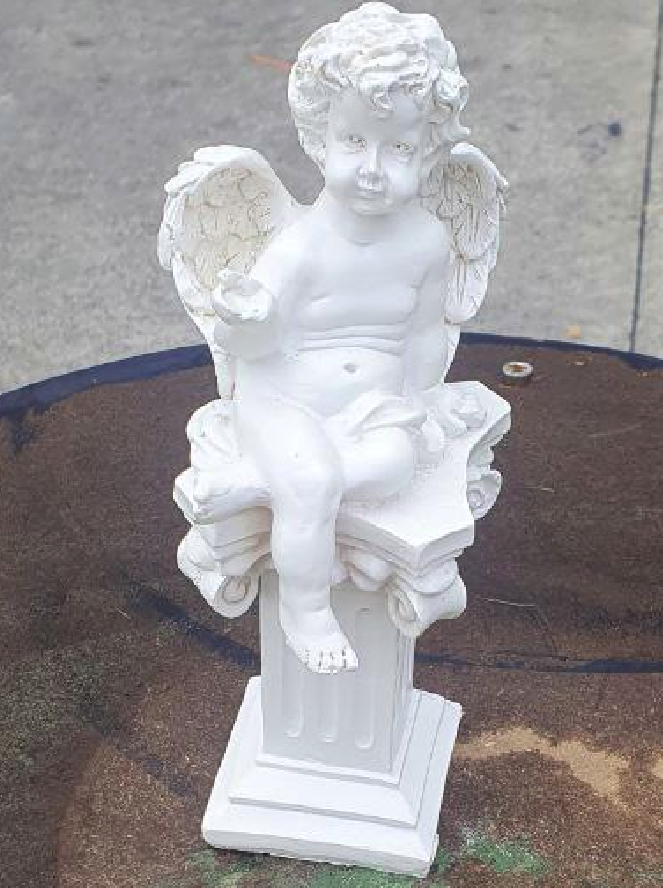
\includegraphics[keepaspectratio,width=0.35\textwidth]{angel}
\end{figure}

119 photos of it were collected, all around it and at three different heights. The 3D model was obtained with Zephyr after the following steps:
\begin{itemize}
\item Sparse point cloud generation, using the 'Human body' and 'High details' presets.
\item Dense point cloud generation, using the 'Human body' and 'High details' presets.
\item Mesh generation, using the 'Default' and 'High details' presets.
\item Textured mesh generation, using the 'Default' and 'High details' presets.
\end{itemize}

\begin{figure}[H]
\centering
\begin{minipage}{0.23\textwidth}
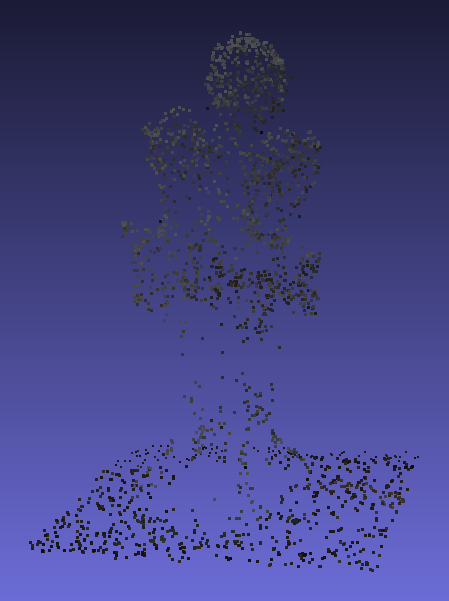
\includegraphics[keepaspectratio,width=0.9\textwidth]{angel_sparse}
\end{minipage}
\begin{minipage}{0.25\textwidth}
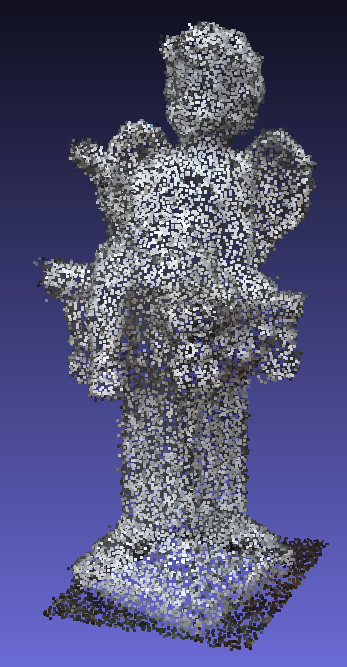
\includegraphics[keepaspectratio,width=0.9\textwidth]{angel_dense}
\end{minipage}
\begin{minipage}{0.25\textwidth}
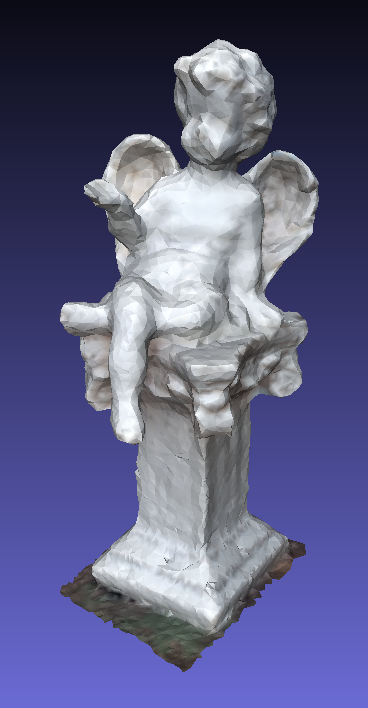
\includegraphics[keepaspectratio,width=0.9\textwidth]{angel_mesh}
\end{minipage}
\begin{minipage}{0.25\textwidth}
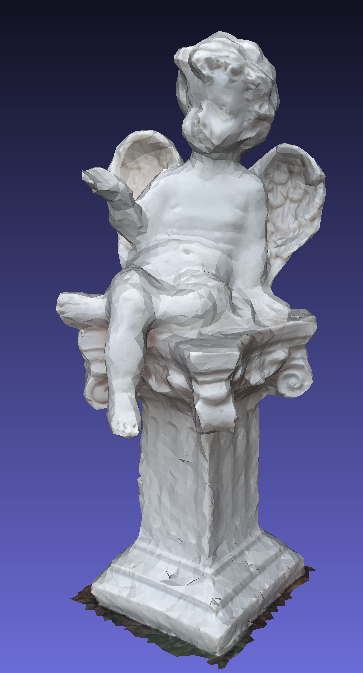
\includegraphics[keepaspectratio,width=0.9\textwidth]{angel_textured_mesh}
\end{minipage}
\caption{From left to right: sparse point cloud, dense point cloud, mesh and textured mesh.}
\end{figure}

\section{Assignment 2}

\subsection{Implement in MATLAB the trapezoidal trajectory taking into account the different constraints.}

The general expression for a trapezoidal velocity profile is:

\begin{equation*}
q(t)=\begin{cases}
q_i+\dot q_i(t-t_i)+\frac{\dot q_c-\dot q_i}{2t_a}(t-t_i)^2 & t_i\leq t\leq t_a+t_i\\
q_i+\dot q_i\frac{t_a}{2}+\dot q_c(t-t_i-\frac{t_a}{2})^2 & t_a+t_i\leq t\leq t_f-t_d\\
q_f-\dot q_f(t_f-t)-\frac{\dot q_c-\dot q_f}{2t_d}(t_f-t)^2 & t_f-t_d\leq t\leq t_f
\end{cases}
\end{equation*}

If the initial and final velocities are null, then $t_a=t_d=t_c$.

If $\dot q_i=\dot q_f=0$ then the possible constraints are:
\begin{itemize}
\item $t_c$:
\begin{equation*}
\ddot q_c = \frac{q_f-q_i}{t_ct_f-t_c^2}\;\;\;\;\dot q_c=\ddot q_ct_c
\end{equation*}
\item $\ddot q_c$:
\begin{equation*}
t_c=\frac{t_f}{2}-\frac{1}{2}\sqrt{\frac{t_f^2\ddot q_c-4(q_f-q_i)}{\ddot q_c}}\;\;\;\;\dot q_c=\ddot q_ct_c
\end{equation*}
\item $\dot q_c$:
\begin{equation*}
t_c=\frac{q_i-q_f+\dot q_ct_f}{\dot q_c}\;\;\;\;\ddot q_c = \frac{\dot q_c^2}{q_i-q_f+\dot q_ct_f}
\end{equation*}
\item $\ddot q_c,\dot q_c$:
\begin{equation*}
t_c=\frac{\dot q_c}{\ddot q_c}\;\;\;\;t_f=\frac{\dot q_c^2+\ddot q_c(q_f-q_i)}{\dot q_c\ddot q_c}
\end{equation*}
\end{itemize}

In all cases the feasibility condition is that $2t_c\leq t_f-t_i$.

If $\dot q_i,\dot q_f\neq 0$ the possible constraints are:

\begin{itemize}
\item $\ddot q_{c,max}$:
\begin{equation*}
\dot q_c = \frac{1}{2}(\dot q_i+\dot q_f+\ddot q_{c,max}\Delta T+\sqrt{\ddot q_{c,max}^2\Delta T^2-4\ddot q_{c,max}\Delta q+2\ddot q_{c,max}(\dot q_i+\dot q_f)\Delta T-(\dot q_i-\dot q_f)^2}\;\;\;\;\;t_a=\frac{\dot q_c-\dot q_i}{\ddot q_{c,max}}\;t_d=\frac{\dot q_c-\dot q_f}{\ddot q_{c,max}}
\end{equation*}

The trajectory is feasible when the argument of the square root is positive, and when the maximum acceleration satisfies:

\begin{equation*}
\ddot q_{c,max}\Delta q>\frac{\abs{\dot q_i^2-\dot q_f^2}}{2}\;\;\;\ddot q_{c,max}\geq\ddot q_{c,lim}=\frac{2\Delta q-(\dot q_i-\dot q_f)\Delta T+\sqrt{4\Delta q^2-4\Delta q(\dot q_i+\dot q_f)\Delta T+2(\dot q_i^2+\dot q_f^2)\Delta T^2}}{\Delta T^2}
\end{equation*}

when $\ddot q_{c,max}=\ddot q_{c,lim}$ there is no constant velocity phase.
\item $\ddot q_{max},\dot q_{max}$:
First we compute the condition:
\begin{equation*}
\ddot q_{c,max}\Delta q\gtreqless\dot q_{c,max}^2-\frac{\dot q_i^2+\dot q_f^2}{2}
\end{equation*}

If the above is $>$ then:

\begin{equation*}
\dot q_c=\dot q_{c,max}\;\;\;t_a=\frac{\dot q_{c,max}-\dot q_i}{\ddot q_{c,max}}\;\;\;t_d=\frac{\dot q_{c,max}-\dot q_f}{\ddot q_{c,max}}\;\;\;\Delta T=\frac{\Delta q\ddot q_{c,max}+\dot q_{c,max}^2}{\ddot q_{c,max}\dot q_{c,max}}
\end{equation*}

If the above is $\leq$ then:
\begin{equation*}
\dot q_c=\dot q_{c,lim}=\sqrt{\ddot q_{c,max}\Delta q+\frac{\dot q_i^2+\dot q_f^2}{2}}<\dot q_{c,max}\;\;\;t_a=\frac{\dot q_{c,lim}-\dot q_i}{\ddot q_{c,max}}\;\;\;t_d=\frac{\dot q_{c,lim}-\dot q_f}{\ddot q_{c,max}}
\end{equation*}
\end{itemize}

\begin{figure}
\begin{minipage}{0.333\textwidth}
\centering
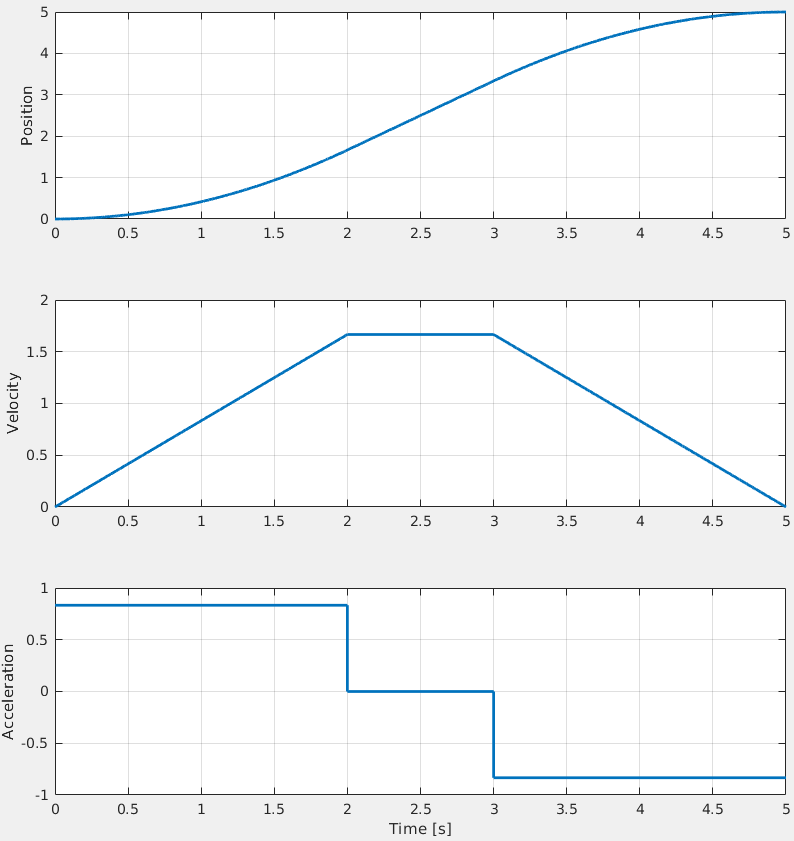
\includegraphics[keepaspectratio,width=\textwidth]{trap_1}
\caption{$t_c=2s$}
\label{fig:trap_1}
\end{minipage}
\begin{minipage}{0.333\textwidth}
\centering
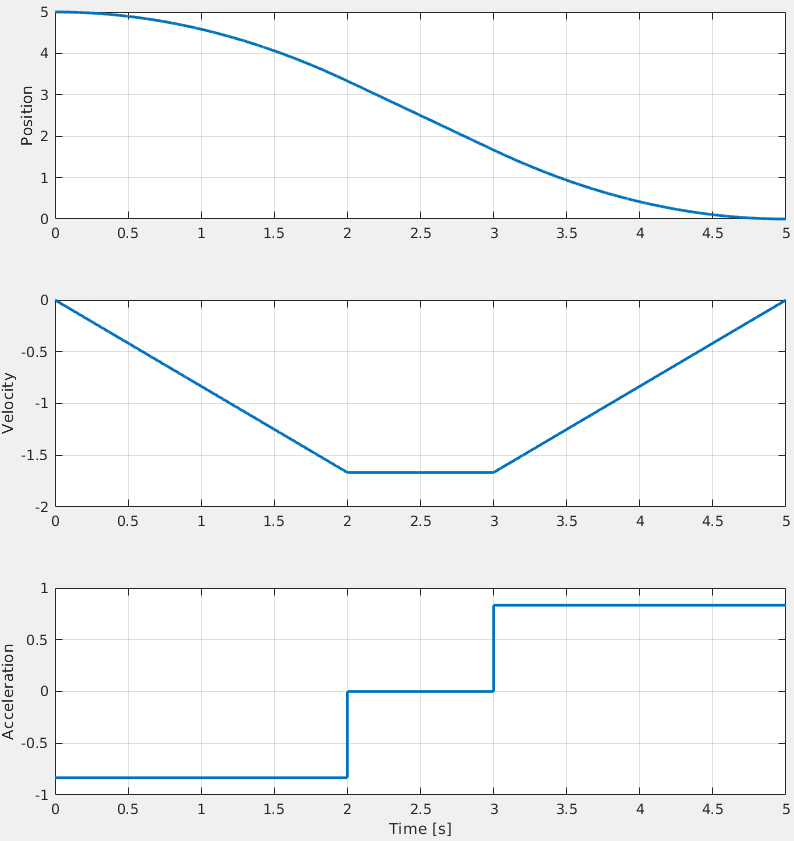
\includegraphics[keepaspectratio,width=\textwidth]{trap_2}
\caption{$t_c=2s, q_i>q_f$}
\label{fig:trap_2}
\end{minipage}
\begin{minipage}{0.333\textwidth}
\centering
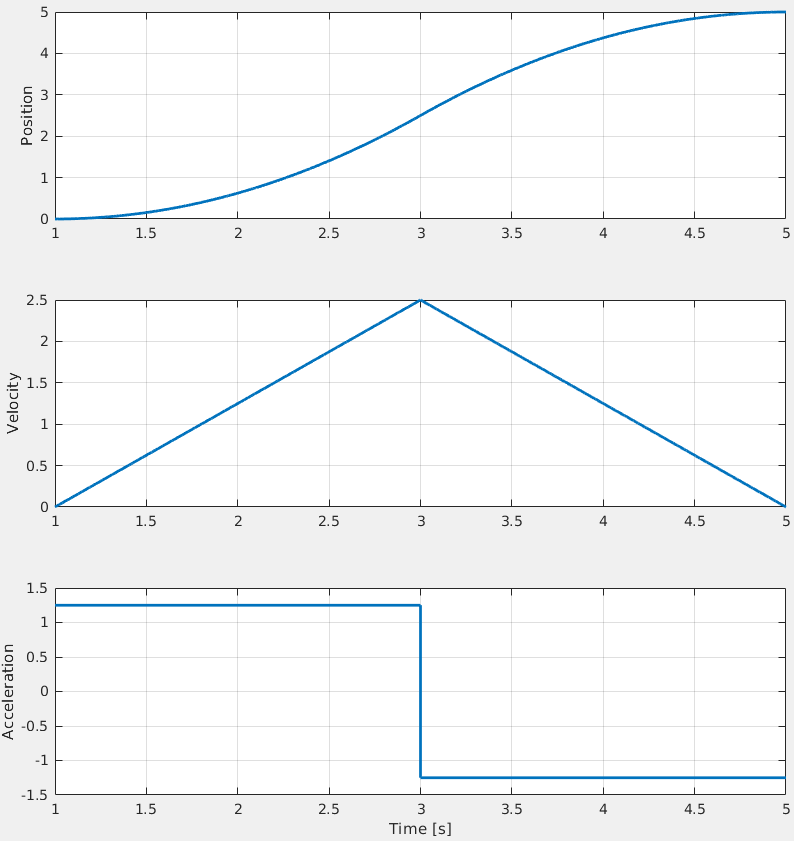
\includegraphics[keepaspectratio,width=\textwidth]{trap_3}
\caption{$t_c=2s, t_i\neq 0$}
\label{fig:trap_3}
\end{minipage}
\end{figure}

\begin{figure}
\begin{minipage}{0.5\textwidth}
\centering
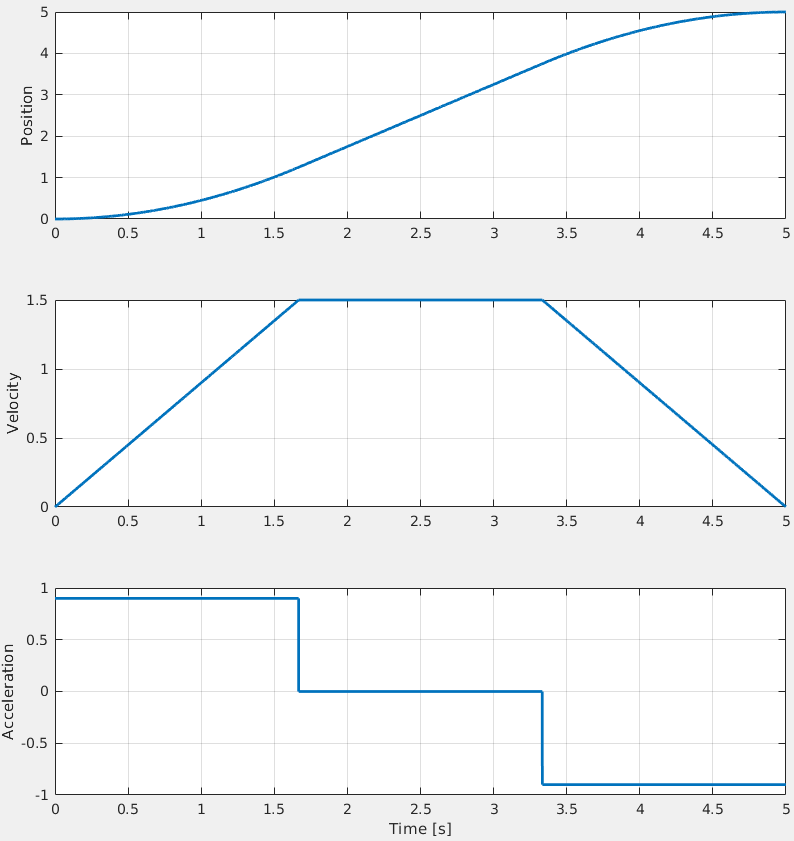
\includegraphics[keepaspectratio,width=\textwidth]{trap_5}
\caption{$v_c=1.5$}
\label{fig:trap_5}
\end{minipage}
\begin{minipage}{0.5\textwidth}
\centering
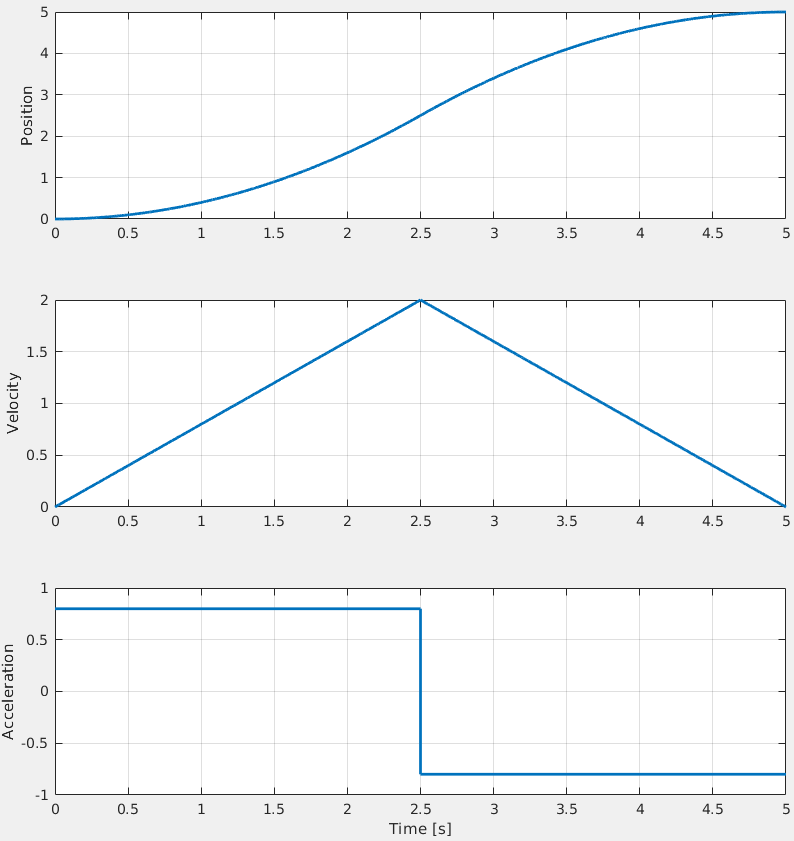
\includegraphics[keepaspectratio,width=\textwidth]{trap_4}
\caption{$v_c=v_{c,lim}=2$}
\label{fig:trap_4}
\end{minipage}
\end{figure}

\begin{figure}
\begin{minipage}{0.5\textwidth}
\centering
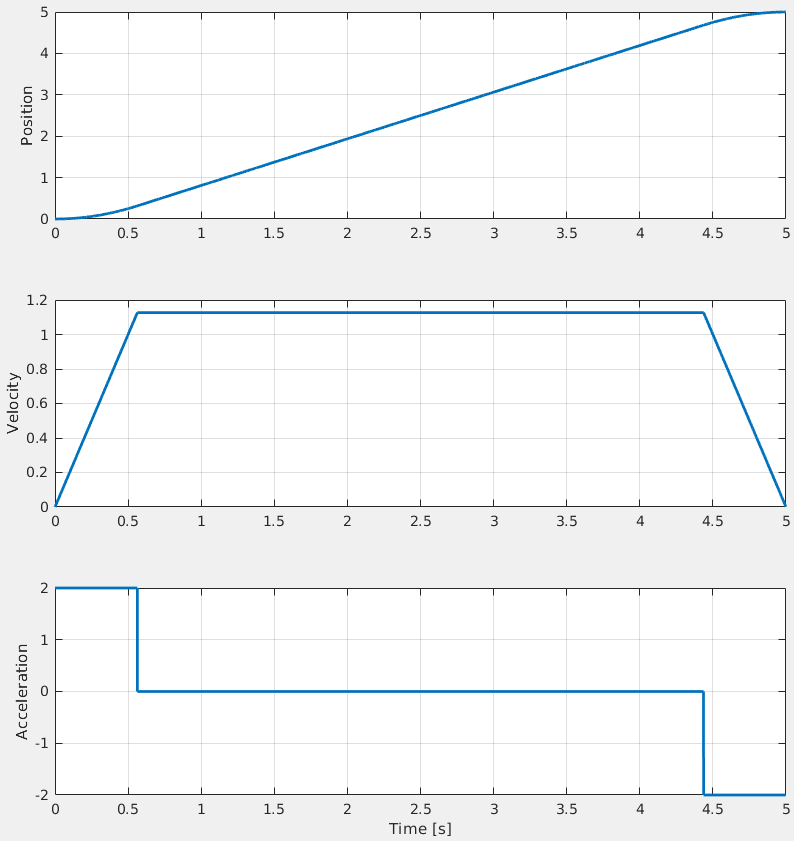
\includegraphics[keepaspectratio,width=\textwidth]{trap_6}
\caption{$a_c=2$}
\label{fig:trap_6}
\end{minipage}
\begin{minipage}{0.5\textwidth}
\centering
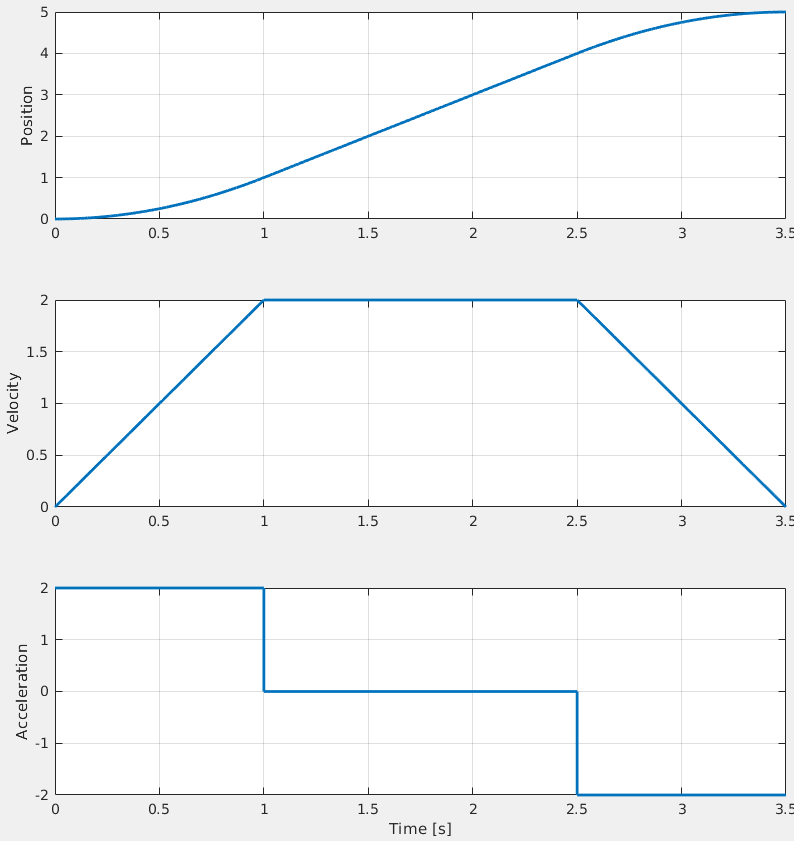
\includegraphics[keepaspectratio,width=\textwidth]{trap_7}
\caption{$a_c,v_c=2$}
\label{fig:trap_7}
\end{minipage}
\end{figure}

\begin{figure}
\begin{minipage}{0.5\textwidth}
\centering
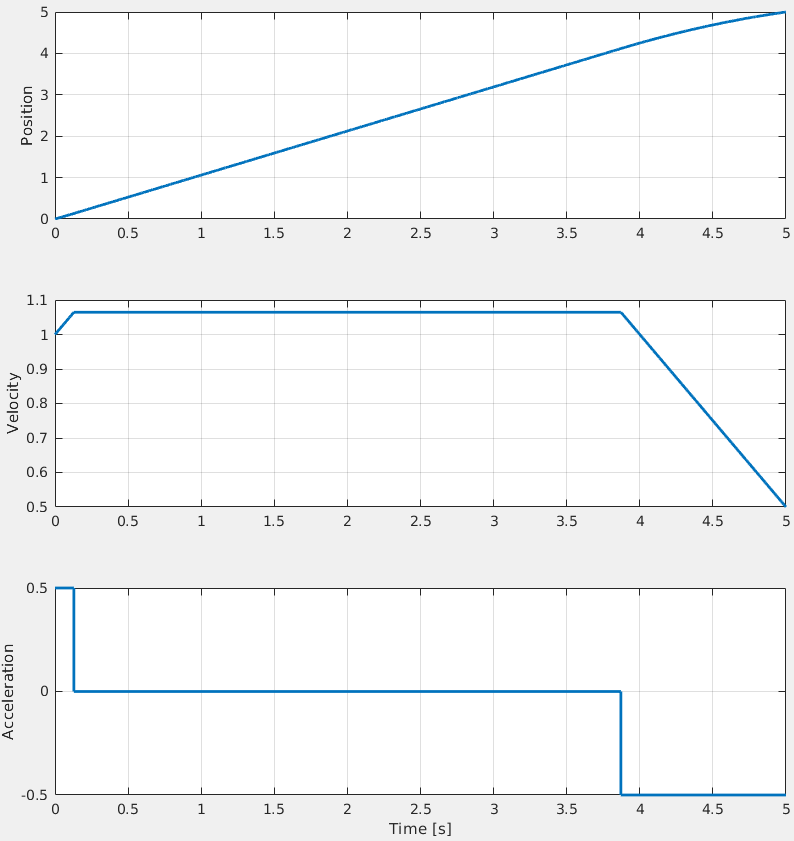
\includegraphics[keepaspectratio,width=\textwidth]{trap_8}
\caption{$\dot q_i=1,\dot q_f=0.5,\ddot q_{max}=0.5$}
\label{fig:trap_8}
\end{minipage}
\begin{minipage}{0.5\textwidth}
\centering
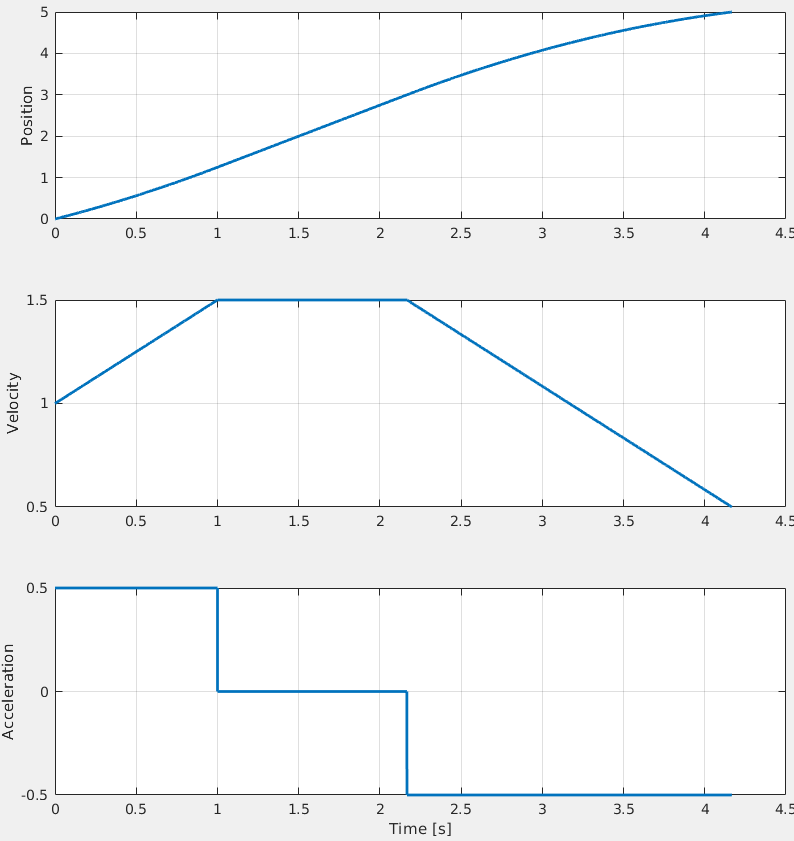
\includegraphics[keepaspectratio,width=\textwidth]{trap_9}
\caption{$\dot q_i=1,\dot q_f=0.5,\dot q_{max}=1.5,\ddot q_{max}=0.5$}
\label{fig:trap_9}
\end{minipage}
\end{figure}

To generate a multipoint trajectory we simply repeat the computation for each consecutive point pair. To improve the resulting velocity and acceleration profiles we can apply an heuristic to assign velocities to each waypoint, so that a less jagged profile is obtained:

\begin{align*}
\dot q(t_i)&=\dot q_i\\
\dot q(t_k)&=\begin{cases}
0 & \text{if }sign(\Delta Q_k)\neq sign(\Delta Q_{k+1})\\
sign(\Delta Q_k)\dot q_{max}& \text{if }sign(\Delta Q_k)= sign(\Delta Q_{k+1})\\
\end{cases}\\
\dot q(t_f)&=\dot q_f
\end{align*}

\begin{figure}
\begin{minipage}{0.5\textwidth}
\centering
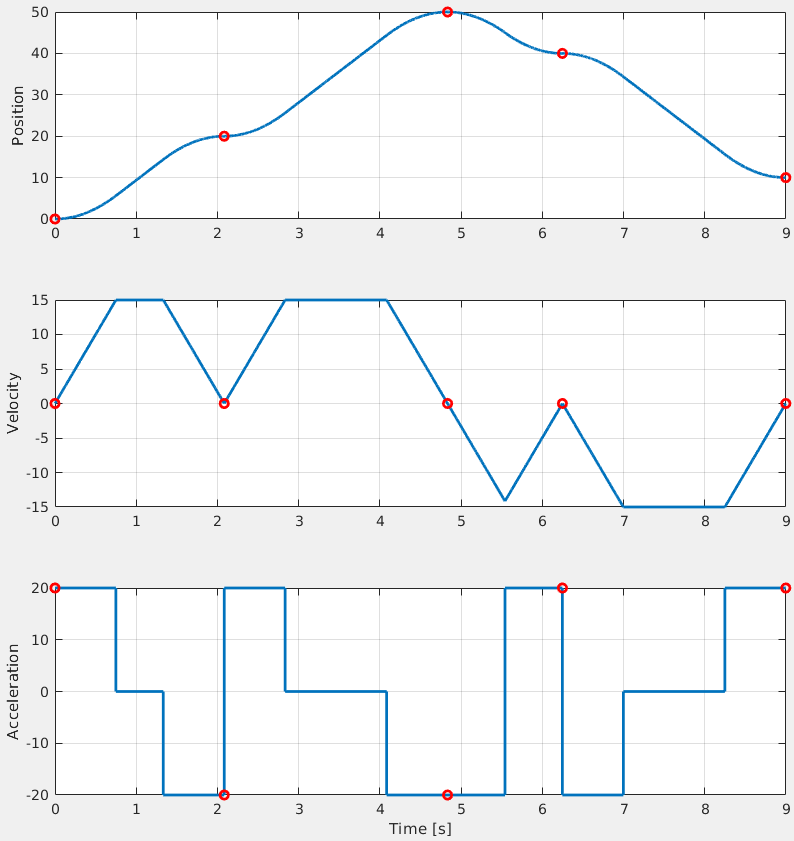
\includegraphics[keepaspectratio,width=\textwidth]{trap_10}
\caption{Multipoint trajectory without velocity heuristic}
\label{fig:trap_10}
\end{minipage}
\begin{minipage}{0.5\textwidth}
\centering
\includegraphics[keepaspectratio,width=\textwidth]{trap_11}
\caption{Multipoint trajectory with velocity heuristic}
\label{fig:trap_11}
\end{minipage}
\end{figure}

\section{Assignment 3}
\subsection{Interpolating polynomials with computed velocities at path points and imposed velocity at initial/final points.}

To implement multipoint trajectories we concatenate cubic splines. The interpolating trajectory is then:

\begin{equation*}
q(t)\coloneqq\{\Pi_k(t),t\in[t_k,t_{k+1}],k=0,\dots,n-1\}
\end{equation*}

where:

\begin{equation*}
\Pi(t)=a_3^k(t-t_k)^3+a_2^k(t-t_k)^2+a_1^k(t-t_k)+a_0^k
\end{equation*}

Fixing velocities on all path points yields:

\begin{equation*}
\begin{cases}
a_0^k&=q_k\\
a_1^k&=\dot q_k\\
a_2^k&=\frac{1}{T_k}\left(\frac{3(q_{k+1}-q_k)}{T_k}-2\dot q_k-\dot q_{k+1}\right)\\
a_3^k&=\frac{1}{T_k^2}\left(\frac{^2(q_{k}-q_{k+1})}{T_k}+\dot q_k+\dot q_{k+1}\right)\\
\end{cases}
\end{equation*}

where $T_k=t_{k+1}-t_k$.

\begin{figure}[h]
\centering
\includegraphics[keepaspectratio,width=0.7\textwidth]{cubic_1}
\caption{Trajectory through $q_k=\begin{bmatrix}
10 & 20 & 0 & 30 & 40
\end{bmatrix}$ at times $t_k=\begin{bmatrix}
0 & 2 & 4 & 8 & 10
\end{bmatrix}$ with \\velocities $\dot q_k=\begin{bmatrix}
0 & 0 & 0 & 5.2 & 0
\end{bmatrix}$}
\end{figure}

\newpage

\subsection{Interpolating polynomials with continuous accelerations at path points and imposed velocity at initial/final points (+ Thomas algorithm)}

Path point velocities are not generally known. We can estimate them with Euler's approximation:

\begin{equation*}
v_k = \frac{q_k-q_{k-1}}{t_k-t_{k-1}}\implies\begin{cases}
\dot q(t_0)&=\dot q_0\\
\dot q(t_k)&=\begin{cases}
0 & \text{if }sign(\Delta Q_k)\neq sign(v_{k+1})\\
\frac{v_k+v_{k+1}}{2} &  \text{if }sign(v_k) =  sign(v_{k+1})\\
\end{cases}\\
\dot q(t_n) &= \dot q_n
\end{cases}
\end{equation*}

Imposing acceleration continuity at path points results in the definition of a linear system $A\dot q=c$, where $A$ is a tridiagonal matrix. Thanks to this property the system can be solved for $\dot q$ efficiently using Thomas' algorithm. Given:

\begin{equation*}
\begin{bmatrix}
b_1 & c_1 & 0 & \dots\\
a_2 & b_2 & c_2 & 0 & \dots\\
0 & \ddots & \ddots & \ddots & 0 & \dots\\
& 0 & a_k & b_k & c_k & 0 & \dots\\
& & 0 & \ddots & \ddots & \ddots & 0 \\
& & & 0 & a_{n-1} & b_{n-1} & c_{n-1}\\
& & & & 0 & a_n & b_n
\end{bmatrix}\begin{bmatrix}
\dot q_1\\\vdots\\\dot  q_k\\\vdots \\ \dot q_n
\end{bmatrix}=\begin{bmatrix}
d_1\\\vdots\\ d_k\\\vdots \\ d_n
\end{bmatrix}
\end{equation*}

Thomas' algorithm is as follows:

\begin{minipage}{0.5\textwidth}
Forward elimination:
\begin{center}
\begin{algorithmic}
    \For{$k=2:1:n$} 
        \State {$m$ $\gets$ {$\frac{a_k}{b_{k-1}}$}}
        \State{$b_k$ $\gets$ {$b_k-mc_{k-1}$}}
        \State{$d_k$ $\gets$ {$d_k-md_{k-1}$}}
    \EndFor
\end{algorithmic}
\end{center}
\end{minipage}
\begin{minipage}{0.5\textwidth}
Backward substitution:
\begin{center}
\begin{algorithmic}
\State{$x_n$ $\gets$ $\frac{d_n}{b_n}$}
    \For{$k=2:1:n$} 
        \State{$x_k$ $\gets$ {$\frac{d_k-c_kx_{k+1}}{b_k}$}}
    \EndFor
\end{algorithmic}
\end{center}
\end{minipage}


\begin{figure}[h]
\begin{minipage}{0.5\textwidth}
\centering
\includegraphics[keepaspectratio,width=\textwidth]{cubic_2}
\caption{Trajectory interpolation with Euler's approximation.}
\end{minipage}
\begin{minipage}{0.5\textwidth}
\centering
\includegraphics[keepaspectratio,width=\textwidth]{cubic_3}
\caption{Trajectory interpolation with continuous accelerations.}
\end{minipage}
\end{figure}

\section{Assignment 4}

\subsection{Image analysis using morphological operators}

2D image analysis can be carried out with the use of morphological operators. Image closing and opening let us remove the background of pictures and isolate the objects within them. More complex operations can then be carried out, inferring for example geometric information on the shapes produced.

Classification used the 'Circularity' property to distinguish between coins and USB stick, as well as the 'MajorAxis' and 'MinorAxis' properties, which were averaged to compute the radius of the coins to detect which was smaller and which was bigger.

\subsubsection{Example 1}

Background removed by opening with a structuring element in the shape of a disk of size 65. Shapes improved by image closing with a structuring element in the shape of a disk of size 25 and by filling holes. Noise removed after image binarization with area opening, removing all shapes with fewer than 50 pixels.

Classification used the 'Circularity' property to distinguish between coins and USB stick, as well as the 'MajorAxis' and 'MinorAxis' properties, which were averaged to compute the radius of the coins to detect which was smaller and which was bigger.

\begin{figure}[h]
\centering
\begin{minipage}{0.45\textwidth}
\includegraphics[keepaspectratio,width=0.9\textwidth]{4_coins_original}
\end{minipage}
\begin{minipage}{0.45\textwidth}
\includegraphics[keepaspectratio,width=0.9\textwidth]{4_coins_shapes}
\end{minipage}
\caption{Original image (left) vs extracted shapes (right).}
\end{figure}
\begin{figure}[h]
\centering
\includegraphics[keepaspectratio,width=0.5\textwidth]{4_coins_labels}
\caption{Labeled image.}
\end{figure}

\newpage

\subsubsection{Example 2}

Background removed by opening with a structuring element in the shape of a disk of size 65. Shapes improved by image closing with a structuring element in the shape of a disk of size 25 and by filling holes. Noise removed after image binarization with area opening, removing all shapes with fewer than 50 pixels.

Classification used the 'Circularity' property to distinguish between washers and bolts. The 'MajorAxis' and 'MinorAxis' properties were averaged to compute the outer radius of the washers, on which a quintic polynomial was fit to determine the relation with the actual inner diameter. For the bolts, the 'Orientation' property was used to align the shapes vertically, so that the bottom part of them, which contains the threaded part, could be extracted. On the extracted shapes, the 'MajorAxis' and 'MinorAxis' properties were extracted and used to fit cubic polynomials to determine, respectively, the bolt length and diameter.

\begin{figure}[h]
\centering
\begin{minipage}{0.3\textwidth}
\includegraphics[keepaspectratio,width=0.9\textwidth]{4_nuts_original}
\end{minipage}
\begin{minipage}{0.3\textwidth}
\includegraphics[keepaspectratio,width=0.9\textwidth]{4_nuts_shapes}
\end{minipage}
\begin{minipage}{0.3\textwidth}
\includegraphics[keepaspectratio,width=0.9\textwidth]{4_nuts_labels}
\end{minipage}
\caption{Original image (left) vs extracted shapes (middle) vs labels (right).}
\end{figure}

\section{Assignment 5}

\subsection{Compute the 3D trajectory (position, velocity, acceleration and jerk) in the picture as
a combination of linear and circular motion primitives and compare it with the
trajectory obtained using one of the multi-point methods.}

\begin{figure}[h]
\centering
\includegraphics[keepaspectratio,width=0.35\textwidth]{3Dtraj_ref}
\caption{3D trajectory - reference.}
\end{figure}

Operational space trajectories can be computed by composing multiple motion primitives. The motion primitives used here are:

\begin{itemize}
\item Rectilinear path:
\begin{equation*}
p(u)=p_i+u(p_f-p_i)\;\;\;\;\;u\in[0,1]
\end{equation*}
\item Circular path:
\begin{equation*}
p(u)=c+Rp'(u)=c+R\begin{bmatrix}
\rho\cos(u)\\\rho\sin(u)\\
0
\end{bmatrix}=c+\begin{bmatrix}
(P-c)' & e_3'\cross(P-c)' & e_3'
\end{bmatrix}\begin{bmatrix}
\rho\cos(u)\\\rho\sin(u)\\
0
\end{bmatrix}\;\;\;\;\;u\in[0,\theta]
\end{equation*}

where $c$ is the position of the center of the circular path, $P$ is the position of the starting point on the circle and $e_3=\begin{bmatrix}
0 & 0 & 1
\end{bmatrix}$.
\end{itemize}

For comparison, a 3D trajectory is computed by computing the smoothing cubic splines along the three directions. The smoothing spline trajectory is also computed with added waypoints to improve the tracking of the position.

\begin{figure}[H]
\centering
\includegraphics[keepaspectratio,width=0.4\textwidth]{3Dtraj}
\caption{3D trajectory - motion primitives vs smoothing splines ($w_k=\infty\forall k$, $\mu=1$).}
\end{figure}

\begin{figure}[h]
\centering
\includegraphics[keepaspectratio,width=0.6\textwidth]{3Dtraj_pos}
\caption{3D trajectory - Position comparison.}
\end{figure}

\begin{figure}[h]
\centering
\includegraphics[keepaspectratio,width=0.9\textwidth]{3Dtraj_profiles}
\caption{3D trajectory - Velocity, acceleration, jerk comparison.}
\end{figure}

\section{Assignment 6}

\subsection{Pose reconstruction pipeline}

\end{document}